% =====================================================================
%  Design of a 32-bit ALU -- Full RTL-to-GDS ASIC Flow
%  Technical documentation (EECS 4612, Digital VLSI)
%
%  Build:  latexmk -pdf main.tex        (or)   pdflatex main.tex  x2
%  See README.md for Overleaf / MiKTeX instructions and figure extraction.
% =====================================================================
\documentclass[11pt,a4paper,oneside]{report}

% =====================================================================
%  preamble.tex -- packages, styles, colours and macros
%  Kept to standard TeX Live / Overleaf packages so the document builds
%  first-try with pdflatex (no shell-escape, no minted).
% =====================================================================

% ---- Encoding & fonts ------------------------------------------------
\usepackage[T1]{fontenc}
\usepackage[utf8]{inputenc}
\usepackage{lmodern}
\usepackage{microtype}

% ---- Page geometry & headers ----------------------------------------
\usepackage[a4paper,margin=1in,headheight=14pt]{geometry}
\usepackage{fancyhdr}
\usepackage{lastpage}

% ---- Maths & symbols -------------------------------------------------
\usepackage{amsmath}
\usepackage{amssymb}
\usepackage{siunitx}
\sisetup{detect-weight=true,detect-family=true}

% ---- Tables ----------------------------------------------------------
\usepackage{booktabs}
\usepackage{array}
\usepackage{multirow}
\usepackage{tabularx}
\usepackage{longtable}
\usepackage{colortbl}
\usepackage{makecell}

% ---- Graphics & figures ---------------------------------------------
\usepackage{graphicx}
\graphicspath{{figures/}}
\usepackage{float}
\usepackage{caption}
\usepackage{subcaption}
\captionsetup{font=small,labelfont=bf}
\captionsetup[sub]{font=footnotesize}

% ---- Colour ----------------------------------------------------------
\usepackage[dvipsnames,table]{xcolor}
\definecolor{accent}{HTML}{1F4E79}      % deep blue -- titles / rules
\definecolor{accentlight}{HTML}{DAE3F3} % light blue -- table headers
\definecolor{arithblk}{HTML}{2E75B6}    % arithmetic datapath
\definecolor{logicblk}{HTML}{548235}    % logic datapath
\definecolor{muxblk}{HTML}{BF8F00}      % multiplexers
\definecolor{padblk}{HTML}{C55A11}      % I/O pads
\definecolor{coreblk}{HTML}{7030A0}     % core
\definecolor{codebg}{HTML}{F6F8FA}
\definecolor{codekw}{HTML}{0000C0}
\definecolor{codecomment}{HTML}{2E8B57}
\definecolor{codestr}{HTML}{A31515}
\definecolor{codenum}{HTML}{B36B00}

% ---- Drawing (TikZ / CircuiTikz) ------------------------------------
\usepackage{tikz}
\usetikzlibrary{arrows.meta,positioning,calc,fit,backgrounds,
                shapes.geometric,shapes.misc,decorations.pathreplacing,
                decorations.markings,chains}
\usepackage[siunitx,RPvoltages]{circuitikz}
\ctikzset{logic ports=ieee}

% Reusable TikZ styles for block diagrams -----------------------------
\tikzset{
  blk/.style     = {draw,thick,rounded corners=2pt,minimum height=9mm,
                     minimum width=16mm,align=center,font=\small},
  arith/.style   = {blk,draw=arithblk,fill=arithblk!12,text=black},
  logic/.style   = {blk,draw=logicblk,fill=logicblk!12,text=black},
  muxb/.style    = {draw=muxblk,fill=muxblk!15,thick,align=center,font=\small},
  core/.style    = {blk,draw=coreblk,fill=coreblk!10,minimum width=26mm,
                     minimum height=18mm},
  pad/.style     = {draw=padblk,fill=padblk!18,thick,minimum width=4mm,
                     minimum height=4mm,inner sep=0pt},
  sig/.style     = {-{Latex[length=2mm]},thick},
  bus/.style     = {-{Latex[length=2.4mm]},line width=1.1pt},
  buslbl/.style  = {font=\scriptsize\ttfamily,inner sep=1pt,fill=white},
  flow/.style    = {blk,minimum width=42mm,minimum height=11mm,
                     draw=accent,fill=accentlight,text=black},
  flowarr/.style = {-{Latex[length=2.6mm]},line width=1pt,draw=accent},
}

% Trapezoidal 4:1 multiplexer symbol: \muxfour{<name>}{<x>}{<y>}
% Draws a downward-tapering trapezoid with four inputs (0..3) on the left.
\newcommand{\muxfour}[3]{%
  \begin{scope}[shift={(#2,#3)}]
    \fill[muxblk!15] (0,0) -- (1.1,-0.35) -- (1.1,-1.85) -- (0,-2.2) -- cycle;
    \draw[muxblk,thick] (0,0) -- (1.1,-0.35) -- (1.1,-1.85) -- (0,-2.2) -- cycle;
    \node[font=\scriptsize] at (0.55,-1.1) {\shortstack{4:1\\MUX}};
    \coordinate (#1-in0) at (0,-0.30);
    \coordinate (#1-in1) at (0,-0.80);
    \coordinate (#1-in2) at (0,-1.30);
    \coordinate (#1-in3) at (0,-1.80);
    \coordinate (#1-out) at (1.1,-1.10);
    \coordinate (#1-sel) at (0.55,-2.03);
  \end{scope}%
}

% ---- Source code listings (Verilog) ---------------------------------
\usepackage{listings}
\lstdefinelanguage{verilogx}[]{Verilog}{%
  morekeywords={wire,reg,logic,always,assign,module,endmodule,input,output,
                inout,begin,end,case,casez,casex,endcase,default,parameter,
                localparam,generate,endgenerate,genvar,for,if,else,posedge,
                negedge}}
\lstdefinestyle{vlog}{
  language=verilogx,
  backgroundcolor=\color{codebg},
  basicstyle=\ttfamily\footnotesize,
  keywordstyle=\color{codekw}\bfseries,
  commentstyle=\color{codecomment}\itshape,
  stringstyle=\color{codestr},
  numberstyle=\tiny\color{gray},
  numbers=left,numbersep=7pt,
  showstringspaces=false,
  breaklines=true,
  frame=single,rulecolor=\color{gray!40},
  framexleftmargin=6pt,
  tabsize=4,
  columns=fullflexible,
  keepspaces=true,
  captionpos=b,
  aboveskip=8pt,belowskip=6pt,
}
\lstset{style=vlog}

% ---- Hyperlinks (load late) -----------------------------------------
\usepackage{hyperref}
\hypersetup{
  colorlinks=true,
  linkcolor=accent,
  citecolor=accent,
  urlcolor=accent,
  filecolor=accent,
  pdftitle={Design of a 32-bit ALU: RTL-to-GDS ASIC Flow},
  pdfauthor={Salwan Aldhahab},
}
\usepackage[nameinlink]{cleveref}
% Give cleveref a name for the listings float (\lstinputlisting labels).
\crefname{lstlisting}{Listing}{Listings}
\Crefname{lstlisting}{Listing}{Listings}
\usepackage{enumitem}
\setlist{nosep,leftmargin=1.5em}

% ---- Header / footer style ------------------------------------------
\pagestyle{fancy}
\fancyhf{}
\renewcommand{\headrulewidth}{0.4pt}
\renewcommand{\footrulewidth}{0pt}
\fancyhead[L]{\small\itshape 32-bit ALU RTL-to-GDS}
\fancyhead[R]{\small\leftmark}
\fancyfoot[C]{\small\thepage}

% Chapter-page style
\fancypagestyle{plain}{%
  \fancyhf{}\renewcommand{\headrulewidth}{0pt}%
  \fancyfoot[C]{\small\thepage}}

% ---- Convenience macros ---------------------------------------------
% Screenshot from the term-project report:
%   \reportfig{<width frac>}{<file>}{<caption>}{<label>}
\newcommand{\reportfig}[4]{%
  \begin{figure}[htbp]\centering
    \includegraphics[width=#1\linewidth]{#2}%
    \caption{#3}\label{#4}%
  \end{figure}}

% Same, with a trailing "(Source: term-project report, Fig. N)" note.
\newcommand{\reportfignote}[5]{%
  \begin{figure}[htbp]\centering
    \includegraphics[width=#1\linewidth]{#2}%
    \caption[#3]{#3\\{\footnotesize\itshape #5}}\label{#4}%
  \end{figure}}

\newcommand{\code}[1]{\texttt{\small #1}}
\newcommand{\sel}{\code{S3\,S2\,S1\,S0}}
\newcommand{\um}{\si{\micro\meter}}
\newcommand{\umsq}{\si{\micro\meter\squared}}

% Signal / bus label helper for prose
\newcommand{\bus}[1]{\texttt{#1}}


\begin{document}

% ---------------------------------------------------------------------
%  Title page
% ---------------------------------------------------------------------
\begin{titlepage}
  \centering
  \vspace*{1.2cm}
  {\color{accent}\rule{\linewidth}{1.4pt}}\\[4pt]
  {\Huge\bfseries Design of a 32-bit ALU}\\[10pt]
  {\LARGE From RTL to GDSII}\\[8pt]
  {\large A Complete Cadence ASIC Implementation Flow\\
   on the GPDK045 \SI{45}{\nano\meter} CMOS Process}\\[6pt]
  {\color{accent}\rule{\linewidth}{1.4pt}}\\[1.4cm]

  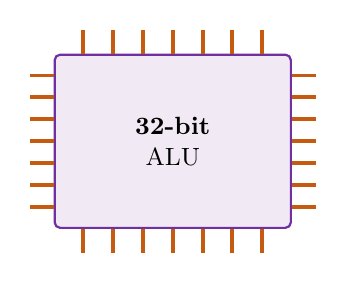
\begin{tikzpicture}[scale=0.95]
    % A small decorative chip icon
    \node[core,minimum width=30mm,minimum height=22mm] (c) {\bfseries 32-bit\\ ALU};
    \foreach \i in {1,...,7}{
      \pgfmathsetmacro{\t}{\i/8}
      \draw[padblk,line width=1.4pt] ($(c.north west)!\t!(c.north east)$)
            -- ++(0,3.2mm);
      \draw[padblk,line width=1.4pt] ($(c.south west)!\t!(c.south east)$)
            -- ++(0,-3.2mm);
      \draw[padblk,line width=1.4pt] ($(c.north west)!\t!(c.south west)$)
            -- ++(-3.2mm,0);
      \draw[padblk,line width=1.4pt] ($(c.north east)!\t!(c.south east)$)
            -- ++(3.2mm,0);
    }
  \end{tikzpicture}\\[1.4cm]

  {\large\bfseries Salwan Aldhahab}\\[2pt]
  {\normalsize Student No.\ 218597963}\\[10pt]
  {\normalsize EECS 4612 --- Digital VLSI}\\[2pt]
  {\normalsize Instructor: Prof.\ Amir M.\ Sodagar}\\[2pt]
  {\normalsize Lassonde School of Engineering, York University}\\[2pt]
  {\normalsize Fall 2025}\\[1.0cm]

  \begin{minipage}{0.86\linewidth}\small\itshape\color{black!70}\centering
    A technical report documenting the design, simulation, synthesis,
    place-and-route, physical verification and full-chip (pad-frame)
    integration of a 32-bit Arithmetic-Logic Unit implemented with a
    bit-slice architecture.
  \end{minipage}

  \vfill
  {\footnotesize Generated as project documentation. Screenshots and
   numerical results are reproduced from the term-project report and the
   Genus/Innovus/Virtuoso output files contained in this repository.}
\end{titlepage}

% ---------------------------------------------------------------------
%  Front matter
% ---------------------------------------------------------------------
\pagenumbering{roman}
\setcounter{page}{2}

\begin{abstract}
\noindent
This report documents the end-to-end ASIC implementation of a 32-bit
Arithmetic-Logic Unit (ALU) taken from register-transfer-level (RTL)
Verilog all the way to a signed-off GDSII layout embedded in an I/O pad
frame. The ALU is built on a \emph{bit-slice} architecture: a fully
verified 1-bit slice is designed first, and thirty-two identical slices
are chained through a ripple carry to form the 32-bit datapath. Two
32-bit realisations are compared---a \emph{structural/hierarchical}
design that instantiates the 1-bit slice, and a single-block
\emph{behavioral} design---and the smaller, faster hierarchical core is
selected for chip integration.

The complete Cadence RTL-to-GDS flow is exercised on the GPDK045
\SI{45}{\nano\meter} CMOS process: functional simulation in Xcelium,
logic synthesis with the \texttt{gsclib045} library in Genus,
place-and-route in Innovus, DRC and connectivity signoff, GDSII export,
and finally pad-frame assembly in Virtuoso. Synthesis results give a core
area of \SI{975.5}{\micro\meter\squared} (367 cells) and a worst-corner
critical path of \SI{9.72}{\nano\second} for the chosen hierarchical
core, dominated---as expected---by the 32-stage ripple-carry chain. Each
flow step is presented with the underlying design decisions, the relevant
schematics, and the tool screenshots and result tables.
\end{abstract}

\tableofcontents
\listoffigures
\listoftables

% ---------------------------------------------------------------------
%  Main matter
% ---------------------------------------------------------------------
\clearpage
\pagenumbering{arabic}
\setcounter{page}{1}

\chapter{Introduction}
\label{ch:intro}

\section{Purpose and scope}
This report documents the design of a 32-bit Arithmetic-Logic Unit (ALU)
and its implementation as a complete integrated circuit using the
industry-standard Cadence RTL-to-GDS design flow. The work was carried
out on the \textbf{GPDK045 \SI{45}{\nano\meter} CMOS} process kit with the
\texttt{gsclib045} standard-cell library. Starting from behavioural and
structural Verilog descriptions, the design is functionally verified,
synthesised to a gate-level netlist, placed and routed into a physical
layout, checked for design-rule and connectivity correctness, exported as
GDSII, and finally embedded inside an I/O pad frame to form a full chip.

The document is written to be read on its own: every flow step is
explained technically, the architectural and implementation decisions are
justified, and each result is shown either as a redrawn schematic
(vector) or as the original tool screenshot captured during the project.

\section{Objectives}
The project exercises the full professional VLSI toolchain. By the end of
the flow the design has been:
\begin{enumerate}
  \item described in synthesisable Verilog RTL (both structural and
        behavioural styles);
  \item simulated and functionally verified against exhaustive test
        vectors in Xcelium;
  \item synthesised to a gate-level netlist with area, power and timing
        reports (Genus);
  \item placed and routed into a physical layout (Innovus);
  \item verified for design rules (DRC) and connectivity;
  \item exported to GDSII; and
  \item integrated into a pad frame to produce the complete chip layout.
\end{enumerate}

\section{The target ALU}
The ALU operates on two 32-bit operands, \bus{A} and \bus{B}, under the
control of a 4-bit function select \sel{} and a carry-in \bus{Cin}. It
produces a 32-bit result \bus{F} and a carry-out \bus{Cout}. Two serial
inputs, \bus{Din,L} and \bus{Din,R}, provide the bits shifted in during
the ``shift left'' and ``shift right'' operations. The top-level
input/output interface is shown in \cref{fig:io}.

\begin{figure}[htbp]
\centering
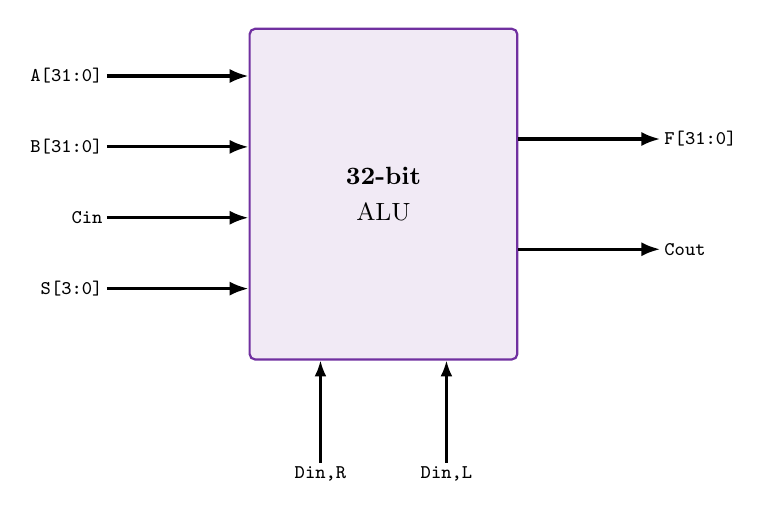
\begin{tikzpicture}[font=\small]
  \node[core,minimum width=34mm,minimum height=42mm] (alu)
        {\bfseries 32-bit\\[2pt] ALU};
  % Left inputs
  \foreach \name/\y in {A[31:0]/1.5, B[31:0]/0.6, Cin/-0.3,
                        {S[3:0]}/-1.2}{
    \draw[bus] ($(alu.west)+(-1.8,\y)$) node[left,buslbl]{\name}
               -- ($(alu.west)+(0,\y)$);
  }
  % Bottom serial inputs
  \draw[sig] ($(alu.south)+(-0.8,-1.3)$) node[below,buslbl]{Din,R}
             -- ($(alu.south)+(-0.8,0)$);
  \draw[sig] ($(alu.south)+(0.8,-1.3)$) node[below,buslbl]{Din,L}
             -- ($(alu.south)+(0.8,0)$);
  % Right outputs
  \draw[bus] ($(alu.east)+(0,0.7)$) -- ($(alu.east)+(1.8,0.7)$)
             node[right,buslbl]{F[31:0]};
  \draw[bus] ($(alu.east)+(0,-0.7)$) -- ($(alu.east)+(1.8,-0.7)$)
             node[right,buslbl]{Cout};
\end{tikzpicture}
\caption{Input/output interface of the target 32-bit ALU. \bus{A} and
\bus{B} are the 32-bit operands, \sel{} the function select, \bus{Cin} the
carry-in; \bus{Din,L}/\bus{Din,R} feed the shift operations; \bus{F} is
the 32-bit result and \bus{Cout} the carry-out.}
\label{fig:io}
\end{figure}

The functional specification of the ALU is given in \cref{tab:func}. The
four select bits are partitioned in hardware: the upper pair
\code{S3\,S2} chooses between the arithmetic unit, the logic unit and the
two shift operations, while the lower pair \code{S1\,S0} chooses the
specific arithmetic or logic function. This partitioning is central to
the architecture and is developed in \cref{ch:arch}.

\begin{table}[htbp]
\centering
\caption{Functional description of the ALU. \bus{Cin} distinguishes the
two operations sharing each arithmetic opcode; ``X'' denotes a don't-care.}
\label{tab:func}
\small
\begin{tabular}{@{}cccc l l@{}}
\toprule
\multicolumn{4}{c}{Select} & \multirow{2}{*}{\bus{Cin}} &
\multirow{2}{*}{Function}\\
\cmidrule(r){1-4}
S3 & S2 & S1 & S0 & & \\
\midrule
\rowcolor{accentlight}\multicolumn{6}{l}{\itshape Arithmetic unit
  (\code{S3\,S2}=00)}\\
0 & 0 & 0 & 0 & 0 & $F = A$ \hfill (transfer $A$)\\
0 & 0 & 0 & 0 & 1 & $F = A+1$ \hfill (increment)\\
0 & 0 & 0 & 1 & 0 & $F = A+B$ \hfill (add)\\
0 & 0 & 0 & 1 & 1 & $F = A+B+1$ \hfill (add with carry)\\
0 & 0 & 1 & 0 & 0 & $F = A+\overline{B}$ \hfill (subtract with borrow)\\
0 & 0 & 1 & 0 & 1 & $F = A+\overline{B}+1$ \hfill (subtract, $A-B$)\\
0 & 0 & 1 & 1 & 0 & $F = A-1$ \hfill (decrement)\\
0 & 0 & 1 & 1 & 1 & $F = A$ \hfill (transfer $A$)\\
\rowcolor{accentlight}\multicolumn{6}{l}{\itshape Logic unit
  (\code{S3\,S2}=01)}\\
0 & 1 & 0 & 0 & X & $F = A \cdot B$ \hfill (AND)\\
0 & 1 & 0 & 1 & X & $F = A + B$ \hfill (OR)\\
0 & 1 & 1 & 0 & X & $F = A \oplus B$ \hfill (XOR)\\
0 & 1 & 1 & 1 & X & $F = \overline{A}$ \hfill (NOT)\\
\rowcolor{accentlight}\multicolumn{6}{l}{\itshape Shift unit
  (\code{S3\,S2}=1X)}\\
1 & 0 & X & X & X & $F = \text{shr } A$ \hfill (shift right one bit)\\
1 & 1 & X & X & X & $F = \text{shl } A$ \hfill (shift left one bit)\\
\bottomrule
\end{tabular}
\end{table}

\section{Bit-slice design methodology}
The ALU is built with a \textbf{bit-slice} (modular) scheme. A bit slice
is a small, identical processing unit that handles a fixed number of bits;
stacking $N$ slices produces an $N$-bit datapath. The advantages exploited
here are:
\begin{itemize}
  \item \textbf{Modularity} --- each slice computes one bit of the result;
  \item \textbf{Scalability} --- the same slice yields an 8-, 16-, 32- or
        64-bit ALU simply by changing the instance count;
  \item \textbf{Reuse} --- one carefully verified slice is replicated,
        rather than designing (and re-verifying) a wide datapath from
        scratch;
  \item \textbf{Reduced complexity} --- verification effort concentrates
        on a single 1-bit cell plus the inter-slice carry connection.
\end{itemize}
Accordingly, the project first designs and fully verifies a \textbf{1-bit
ALU slice} (\cref{ch:arch,ch:part1}), then chains \textbf{thirty-two}
slices into the 32-bit ALU (\cref{ch:part2a}). For comparison, a
functionally equivalent single-block \textbf{behavioural} 32-bit ALU is
also written (\cref{ch:part2b}), and the two are compared on area, power
and speed before one is chosen for chip integration (\cref{ch:compare}).

\chapter{The RTL-to-GDS ASIC Flow}
\label{ch:flow}

This chapter gives the overall methodology --- the sequence of design
steps that turn a Verilog description into a manufacturable layout --- and
the tools and technology used at each stage. The remaining chapters then
apply this flow to the 1-bit slice and to the two 32-bit designs.

\section{Flow overview}
The RTL-to-GDS (or ``RTL-to-GDSII'') flow is the standard digital ASIC
implementation methodology. Design intent is captured at the
register-transfer level and progressively refined --- through synthesis
and physical implementation --- into geometry, while functional and
physical correctness are checked at every hand-off. \Cref{fig:flow}
summarises the steps used in this project and the artefacts produced at
each one.

\begin{figure}[htbp]
\centering
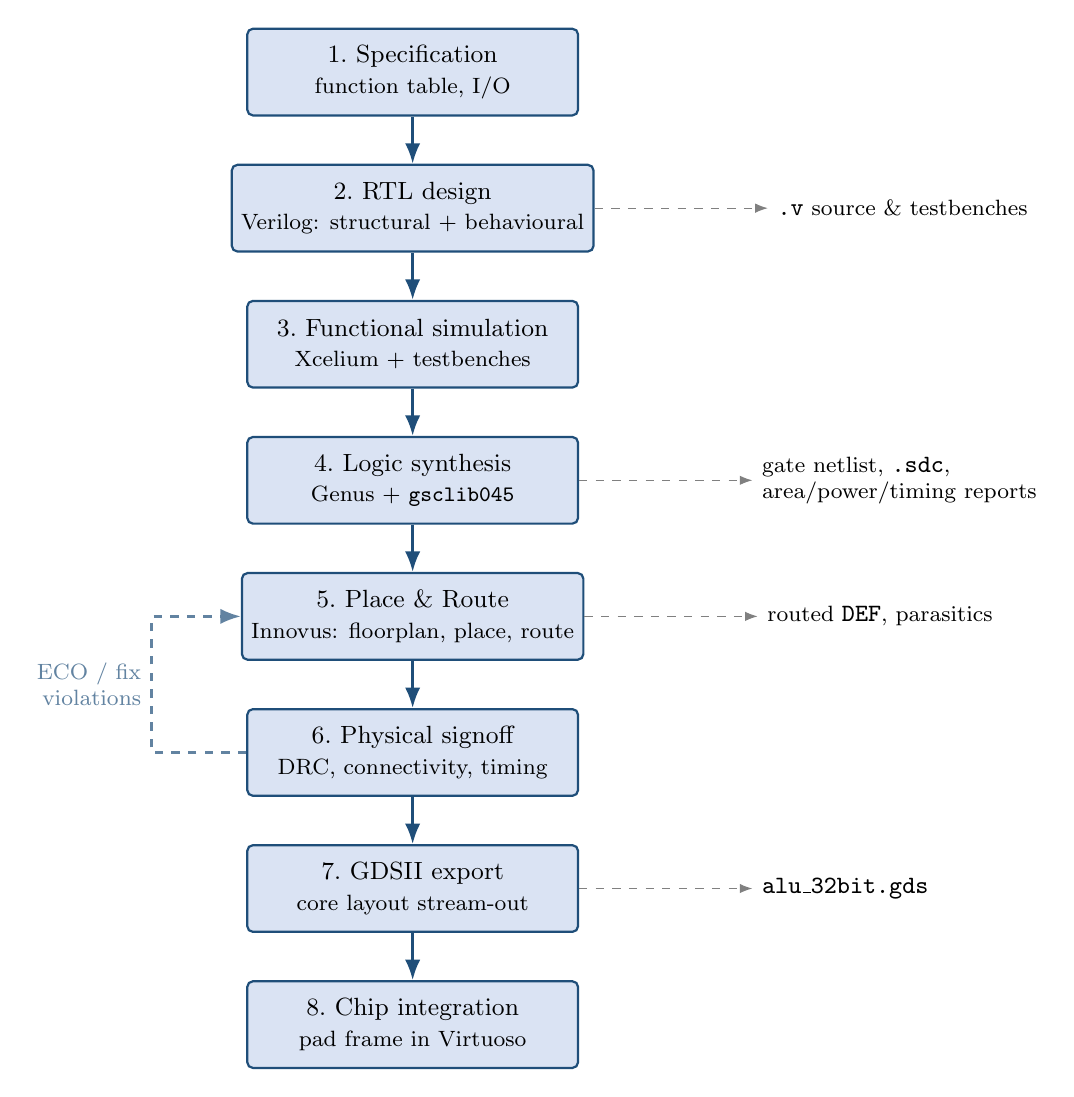
\begin{tikzpicture}[node distance=6mm and 22mm,font=\small]
  \node[flow] (spec) {1.\ Specification\\{\footnotesize function table, I/O}};
  \node[flow,below=of spec] (rtl) {2.\ RTL design\\{\footnotesize Verilog: structural + behavioural}};
  \node[flow,below=of rtl] (sim) {3.\ Functional simulation\\{\footnotesize Xcelium + testbenches}};
  \node[flow,below=of sim] (syn) {4.\ Logic synthesis\\{\footnotesize Genus + \texttt{gsclib045}}};
  \node[flow,below=of syn] (pnr) {5.\ Place \& Route\\{\footnotesize Innovus: floorplan, place, route}};
  \node[flow,below=of pnr] (sign) {6.\ Physical signoff\\{\footnotesize DRC, connectivity, timing}};
  \node[flow,below=of sign] (gds) {7.\ GDSII export\\{\footnotesize core layout stream-out}};
  \node[flow,below=of gds] (chip) {8.\ Chip integration\\{\footnotesize pad frame in Virtuoso}};

  \foreach \a/\b in {spec/rtl,rtl/sim,sim/syn,syn/pnr,pnr/sign,sign/gds,gds/chip}
     \draw[flowarr] (\a) -- (\b);

  % Right-hand annotations (artefacts)
  \node[right=of rtl,align=left,font=\footnotesize] (a1)
       {\code{.v} source \& testbenches};
  \node[right=of syn,align=left,font=\footnotesize] (a2)
       {gate netlist, \code{.sdc},\\ area/power/timing reports};
  \node[right=of pnr,align=left,font=\footnotesize] (a3)
       {routed \code{DEF}, parasitics};
  \node[right=of gds,align=left,font=\footnotesize] (a4)
       {\code{alu\_32bit.gds}};
  \foreach \n/\a in {rtl/a1,syn/a2,pnr/a3,gds/a4}
     \draw[-{Latex[length=1.6mm]},gray,dashed] (\n.east) -- (\a.west);

  % Feedback loop: signoff failures return to place & route / synthesis
  \draw[flowarr,accent!70,dashed]
     (sign.west) -- ++(-1.2,0) |- node[pos=0.25,left,font=\footnotesize,align=right]
        {ECO / fix\\violations} (pnr.west);
\end{tikzpicture}
\caption{The RTL-to-GDS flow applied in this project. Solid arrows show
the forward flow; the dashed feedback path indicates iteration when
signoff checks (timing, DRC, connectivity) fail.}
\label{fig:flow}
\end{figure}

\section{Process technology and libraries}
All implementation uses the Cadence \textbf{GPDK045} generic
\SI{45}{\nano\meter} CMOS process design kit. \Cref{tab:tech} lists the
key technology and library settings that appear throughout the synthesis
and PnR reports.

\begin{table}[htbp]
\centering
\caption{Technology and library configuration.}
\label{tab:tech}
\small
\begin{tabularx}{\linewidth}{@{}l X@{}}
\toprule
Item & Setting \\
\midrule
Process               & Cadence GPDK045, \SI{45}{\nano\meter} bulk CMOS \\
Standard-cell library & \texttt{gsclib045} (LEF: \texttt{gsclib045\_tech.lef},
                        \texttt{gsclib045\_macro.lef}) \\
Timing corner         & \texttt{PVT\_0P9V\_125C}, worst-case
                        \texttt{slow\_vdd1v0} liberty \\
Supply / ground nets  & \texttt{VDD} / \texttt{VSS} \\
Routing pin layer     & Metal~4 (from the pin-assignment file) \\
Multi-mode multi-corner& \texttt{mmmc.view} (setup on slow corner) \\
\bottomrule
\end{tabularx}
\end{table}

Choosing the \emph{slow}, low-voltage, high-temperature corner
(\SI{0.9}{\volt}, \SI{125}{\celsius}) for setup analysis is deliberate: it
represents the worst case for cell delay, so timing that closes here
closes across the operating range. All area/power/timing numbers quoted in
this report are from this corner unless stated otherwise.

\section{Tools used}
\Cref{tab:tools} maps each flow step to the Cadence tool that performs it.

\begin{table}[htbp]
\centering
\caption{Tools used at each stage of the flow.}
\label{tab:tools}
\small
\begin{tabularx}{\linewidth}{@{}l l X@{}}
\toprule
Stage & Tool & Role \\
\midrule
Simulation      & Xcelium (SimVision) & Event-driven verification of RTL against testbenches \\
Synthesis       & Genus 21.17         & RTL $\rightarrow$ gate netlist mapped to \texttt{gsclib045}; area/power/timing \\
Place \& Route  & Innovus             & Floorplan, power, placement, routing, post-route timing \\
Signoff         & Innovus / Pegasus / Assura & DRC and connectivity (LVS-style) checks \\
Chip assembly   & Virtuoso            & Pad-frame placement, I/O wiring, full-chip stream-out \\
\bottomrule
\end{tabularx}
\end{table}

\section{Design flavours implemented}
Because the assignment requires the 32-bit ALU to be built ``in two
ways,'' three distinct RTL designs are carried through the flow:
\begin{description}[leftmargin=2.4em,style=nextline]
  \item[Part 1 --- 1-bit ALU] the bit-slice cell, verified in isolation
        and taken through synthesis and PnR on its own
        (\cref{ch:part1}).
  \item[Part 2a --- 32-bit hierarchical] a \emph{structural} design that
        instantiates thirty-two 1-bit slices and connects their carries in
        a ripple chain (\cref{ch:part2a}).
  \item[Part 2b --- 32-bit behavioural] a single-module design that models
        the operations directly on 32-bit vectors with a \code{casez}
        statement (\cref{ch:part2b}).
\end{description}
The two 32-bit cores are compared in \cref{ch:compare}; the smaller and
faster one is streamed out and dropped into the pad frame in
\cref{ch:pad}.

\chapter{Architecture of the 1-bit ALU Slice}
\label{ch:arch}

The whole design rests on one carefully built block: the 1-bit ALU slice.
This chapter develops that slice bottom-up --- full adder, multiplexer,
arithmetic unit, logic unit --- and shows how they compose into the
complete slice, giving the reasoning behind each choice. Every schematic
here is redrawn as vector art; the corresponding Verilog is listed
alongside so the figure and the code can be read together.

\section{Structural decomposition}
The 1-bit slice is partitioned into three cooperating sub-blocks,
selected by the two halves of \sel{}:
\begin{itemize}
  \item an \textbf{arithmetic circuit} that produces the adder result
        $D_i$ and carry-out, controlled by \code{S1\,S0};
  \item a \textbf{logic circuit} that produces the bitwise result $E_i$,
        also controlled by \code{S1\,S0}; and
  \item an output \textbf{4:1 multiplexer} that selects between $D_i$,
        $E_i$, and the two shifted versions of $A$, controlled by
        \code{S3\,S2}.
\end{itemize}
\Cref{fig:alu1top} shows the composition. The key architectural decision
is this two-level select: \code{S3\,S2} picks the \emph{class} of
operation (arithmetic / logic / shift) at the output mux, while
\code{S1\,S0} picks the \emph{specific} operation inside the arithmetic
and logic units. This lets both internal units run in parallel and share
the same lower select bits, and it is exactly what makes the slice
replicable --- no bit position needs special-case control.

\begin{figure}[htbp]
\centering
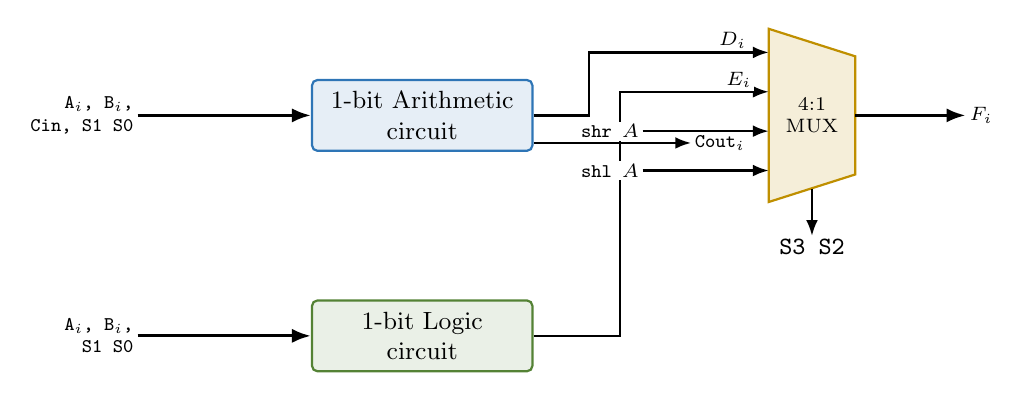
\begin{tikzpicture}[font=\small]
  % Arithmetic + logic blocks
  \node[arith,minimum width=28mm] (ar) at (0,1.4)
        {1-bit Arithmetic\\ circuit};
  \node[logic,minimum width=28mm] (lo) at (0,-1.4)
        {1-bit Logic\\ circuit};

  % Output mux
  \muxfour{om}{4.4}{2.5}

  % Bundled inputs into the two units
  \draw[bus] ($(ar.west)+(-2.2,0)$)
        node[left,buslbl,align=right]{A$_i$, B$_i$,\\ Cin, S1 S0}
        -- (ar.west);
  \draw[bus] ($(lo.west)+(-2.2,0)$)
        node[left,buslbl,align=right]{A$_i$, B$_i$,\\ S1 S0}
        -- (lo.west);

  % arithmetic -> mux in0, logic -> mux in1
  \draw[sig] (ar.east) -- ($(ar.east)+(0.7,0)$)
        |- node[pos=0.9,above,buslbl]{$D_i$} (om-in0);
  \draw[sig] (lo.east) -- ($(lo.east)+(1.1,0)$)
        |- node[pos=0.9,above,buslbl]{$E_i$} (om-in1);
  % shifts into mux
  \draw[sig] ($(om-in2)+(-1.6,0)$) node[left,buslbl]{shr $A$} -- (om-in2);
  \draw[sig] ($(om-in3)+(-1.6,0)$) node[left,buslbl]{shl $A$} -- (om-in3);
  % select
  \draw[sig] (om-sel) -- ($(om-sel)+(0,-0.6)$) node[below,buslbl]{\code{S3 S2}};

  % output + cout
  \draw[bus] (om-out) -- ($(om-out)+(1.4,0)$) node[right,buslbl]{$F_i$};
  \draw[sig] ($(ar.east)+(0,-0.35)$) -- ($(ar.east)+(2.0,-0.35)$)
        node[right,buslbl]{Cout$_i$};
\end{tikzpicture}
\caption{Top-level datapath of the 1-bit ALU slice. \code{S1\,S0} selects
the function inside the arithmetic and logic units; \code{S3\,S2} selects
the output class (arithmetic $D_i$, logic $E_i$, shift-right or
shift-left of $A$) at the output 4:1 multiplexer.}
\label{fig:alu1top}
\end{figure}

\lstinputlisting[style=vlog,caption={\texttt{alu\_1bit.v} --- top-level
1-bit slice.},label={lst:alu1}]{rtl/alu_1bit.v}

Note in \cref{lst:alu1} that the shift inputs to the output mux
(\code{a\_shr\_1bit}, \code{a\_shl\_1bit}) are derived locally from
\code{a\_i}. In a single bit this is a placeholder for the inter-slice
shift wiring that is realised at the 32-bit level (\cref{ch:part2a}).

\section{The 4:1 multiplexer}
Every selection point in the slice --- inside the arithmetic unit, inside
the logic unit, and at the output --- is a 4:1 multiplexer. A single
parameter-free \code{mux4x1} module is therefore written once and reused,
which is a small but real instance of the reuse principle behind the whole
design.

\begin{figure}[htbp]
\centering
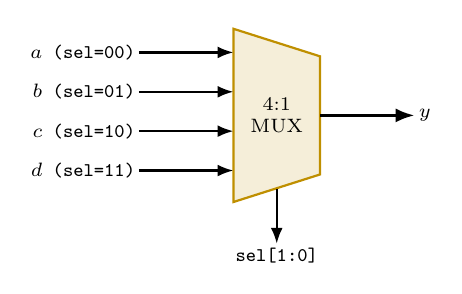
\begin{tikzpicture}[font=\small]
  \muxfour{m}{0}{1.1}
  \draw[sig] ($(m-in0)+(-1.2,0)$) node[left,buslbl]{$a$ (sel=00)} -- (m-in0);
  \draw[sig] ($(m-in1)+(-1.2,0)$) node[left,buslbl]{$b$ (sel=01)} -- (m-in1);
  \draw[sig] ($(m-in2)+(-1.2,0)$) node[left,buslbl]{$c$ (sel=10)} -- (m-in2);
  \draw[sig] ($(m-in3)+(-1.2,0)$) node[left,buslbl]{$d$ (sel=11)} -- (m-in3);
  \draw[bus] (m-out) -- ++(1.2,0) node[right,buslbl]{$y$};
  \draw[sig] (m-sel) -- ++(0,-0.7) node[below,buslbl]{sel[1:0]};
\end{tikzpicture}
\caption{The reusable 4:1 multiplexer. The two select bits route one of
the four data inputs to the output.}
\label{fig:mux}
\end{figure}

\lstinputlisting[style=vlog,caption={\texttt{mux4x1.v} --- reused 4:1
multiplexer.},label={lst:mux}]{rtl/mux4x1.v}

\section{The full adder}
The arithmetic unit is built around a single-bit full adder implementing
\begin{align}
  \text{sum}  &= A \oplus B \oplus C_{in}, \label{eq:fasum}\\
  \text{cout} &= (A\cdot B) + \bigl(C_{in}\cdot(A\oplus B)\bigr).
  \label{eq:facout}
\end{align}
\Cref{fig:fa} is the gate-level realisation of
\cref{eq:fasum,eq:facout}: two XOR gates form the sum, and an
AND-AND-OR network forms the carry, sharing the first XOR ($A\oplus B$)
between the two halves.

\begin{figure}[htbp]
\centering
\begin{circuitikz}[scale=0.9,transform shape,font=\small]
  % Level-1 gates
  \node[xor port]  (x1) at (2.4,3.0) {};
  \node[and port]  (a1) at (2.4,0.6) {};
  % Level-2 gates
  \node[xor port]  (x2) at (5.6,2.6) {};
  \node[and port]  (a2) at (5.6,1.4) {};
  \node[or port]   (o1) at (8.2,1.0) {};

  % Primary inputs
  \node (A) at (0,3.3) {\code{A}};
  \node (B) at (0,2.5) {\code{B}};
  \node (C) at (0,1.0) {\code{Cin}};

  % A,B into x1
  \draw (A) -- (x1.in 1);
  \draw (B) -- (x1.in 2);
  % A,B into a1
  \draw (A) -- ++(0.6,0) |- (a1.in 1);
  \draw (B) -- ++(0.4,0) |- (a1.in 2);
  % x1 -> t1 node, fan to x2.in1 and a2.in1
  \draw (x1.out) -- ++(0.4,0) coordinate (t1);
  \node[circle,fill,inner sep=1pt] at (t1) {};
  \draw (t1) |- (x2.in 1);
  \draw (t1) |- (a2.in 1);
  % Cin -> x2.in2 and a2.in2
  \draw (C) -| ($(x2.in 2)+(-0.6,0)$) -- (x2.in 2);
  \draw (C) -- ++(3.6,0) |- (a2.in 2);
  % sum output
  \draw (x2.out) -- ++(0.8,0) node[right]{\code{sum}\,$=D_i$};
  % carry network
  \draw (a1.out) -- ++(0.5,0) |- (o1.in 1);
  \draw (a2.out) -- (o1.in 2);
  \draw (o1.out) -- ++(0.6,0) node[right]{\code{cout}\,$=$\,Cout$_i$};
\end{circuitikz}
\caption{Gate-level full adder. The shared term $A\oplus B$ feeds both the
sum's second XOR and the carry's second AND, minimising gate count.}
\label{fig:fa}
\end{figure}

\lstinputlisting[style=vlog,caption={\texttt{full\_adder.v}.},
label={lst:fa}]{rtl/full_adder.v}

\section{The arithmetic circuit}
The arithmetic unit turns the single adder into eight operations by
choosing \emph{what the adder's second operand is}. A 4:1 multiplexer
drives the adder's $B$ input with one of four values selected by
\code{S1\,S0}, and \bus{Cin} then distinguishes the two operations within
each opcode (\cref{tab:arithmux}). \Cref{fig:arith} shows the structure.

\begin{table}[htbp]
\centering
\caption{Operand-select encoding of the arithmetic unit. Feeding the adder
$0$, $B$, $\overline{B}$ or $1$ (with the carry-in) realises transfer,
add, subtract and increment/decrement.}
\label{tab:arithmux}
\small
\begin{tabular}{@{}cc l l@{}}
\toprule
\code{S1} & \code{S0} & Adder $B$-input & Resulting function ($C_{in}=0/1$)\\
\midrule
0 & 0 & $0$              & $A$ \,/\, $A+1$ \\
0 & 1 & $B$              & $A+B$ \,/\, $A+B+1$ \\
1 & 0 & $\overline{B}$   & $A+\overline{B}$ \,/\, $A+\overline{B}+1=A-B$ \\
1 & 1 & $1$              & $A-1$ \,/\, $A$ \\
\bottomrule
\end{tabular}
\end{table}

\begin{figure}[htbp]
\centering
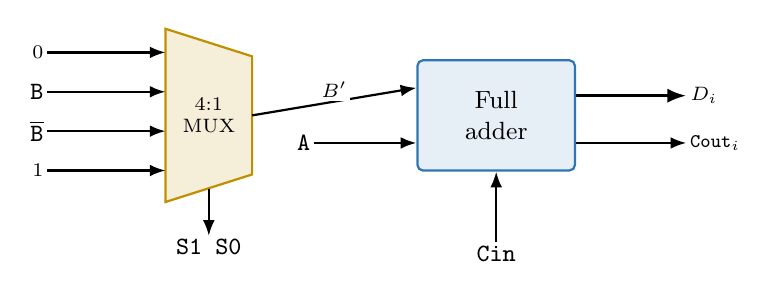
\begin{tikzpicture}[font=\small]
  \muxfour{bm}{0}{1.1}
  \draw[sig] ($(bm-in0)+(-1.5,0)$) node[left,buslbl]{$0$} -- (bm-in0);
  \draw[sig] ($(bm-in1)+(-1.5,0)$) node[left,buslbl]{\code{B}} -- (bm-in1);
  \draw[sig] ($(bm-in2)+(-1.5,0)$) node[left,buslbl]{$\overline{\code{B}}$} -- (bm-in2);
  \draw[sig] ($(bm-in3)+(-1.5,0)$) node[left,buslbl]{$1$} -- (bm-in3);
  \draw[sig] (bm-sel) -- ++(0,-0.6) node[below,buslbl]{\code{S1 S0}};

  \node[blk,arith,minimum width=20mm,minimum height=14mm] (fa) at (4.2,0)
        {Full\\ adder};
  \draw[sig] (bm-out) -- ($(fa.west)+(0,0.35)$)
        node[midway,above,buslbl]{$B'$};
  \draw[sig] ($(fa.west)+(-1.3,-0.35)$) node[left,buslbl]{\code{A}}
        -- ($(fa.west)+(0,-0.35)$);
  \draw[sig] ($(fa.south)+(0,-0.9)$) node[below,buslbl]{\code{Cin}}
        -- (fa.south);
  \draw[bus] ($(fa.east)+(0,0.25)$) -- ($(fa.east)+(1.4,0.25)$)
        node[right,buslbl]{$D_i$};
  \draw[sig] ($(fa.east)+(0,-0.35)$) -- ($(fa.east)+(1.4,-0.35)$)
        node[right,buslbl]{Cout$_i$};
\end{tikzpicture}
\caption{Arithmetic circuit: a 4:1 multiplexer selects the adder's second
operand ($0$, $B$, $\overline{B}$ or $1$); the full adder then combines it
with $A$ and the carry-in. Subtraction is two's-complement:
$\overline{B}+C_{in}$.}
\label{fig:arith}
\end{figure}

\lstinputlisting[style=vlog,caption={\texttt{arithmetic\_circuit.v}.},
label={lst:arith}]{rtl/arithmetic_circuit.v}

\paragraph{Design decision --- two's-complement subtraction.}
Rather than build a dedicated subtractor, subtraction reuses the same
adder: $A-B = A + \overline{B} + 1$. Selecting $\overline{B}$ at the mux
and driving $C_{in}=1$ yields $A-B$, while $C_{in}=0$ yields the
subtract-with-borrow result $A+\overline{B}$. This is why the functional
table pairs each opcode with a \bus{Cin} value, and it keeps the slice to
a single adder.

\section{The logic circuit}
The logic unit computes the four bitwise functions of $A$ and $B$ in
parallel and selects one with a 4:1 multiplexer on \code{S1\,S0}
(\cref{fig:logic}).

\begin{figure}[htbp]
\centering
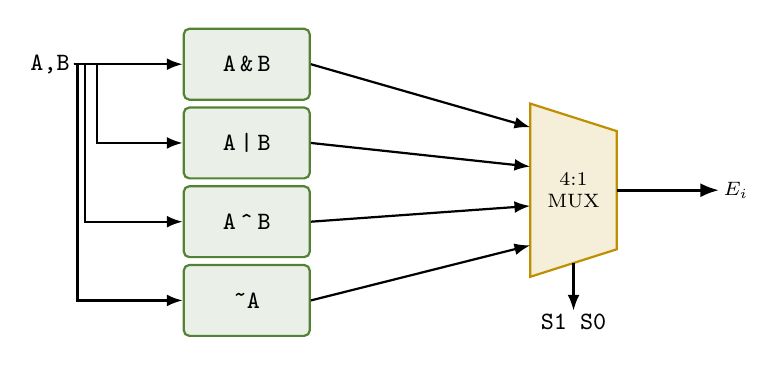
\begin{tikzpicture}[font=\small]
  \node[logic] (g0) at (0,1.6) {\code{A\,\&\,B}};
  \node[logic] (g1) at (0,0.6) {\code{A\,|\,B}};
  \node[logic] (g2) at (0,-0.4){\code{A\,\^{}\,B}};
  \node[logic] (g3) at (0,-1.4){\code{\~{}A}};
  \muxfour{lm}{3.6}{1.1}
  \draw[sig] (g0.east) -- (lm-in0);
  \draw[sig] (g1.east) -- (lm-in1);
  \draw[sig] (g2.east) -- (lm-in2);
  \draw[sig] (g3.east) -- (lm-in3);
  \draw[sig] (lm-sel) -- ++(0,-0.6) node[below,buslbl]{\code{S1 S0}};
  \draw[bus] (lm-out) -- ++(1.3,0) node[right,buslbl]{$E_i$};
  \draw[sig] (-2.2,1.6) node[left,buslbl]{\code{A,B}} -- (g0.west);
  \draw[sig] (-2.2,1.6) -- ++(0.3,0) |- (g1.west);
  \draw[sig] (-2.2,1.6) -- ++(0.15,0) |- (g2.west);
  \draw[sig] (-2.2,1.6) -- ++(0.05,0) |- (g3.west);
\end{tikzpicture}
\caption{Logic circuit: AND, OR, XOR and NOT are computed in parallel and
a 4:1 multiplexer selects the required one.}
\label{fig:logic}
\end{figure}

\lstinputlisting[style=vlog,caption={\texttt{logic\_circuit.v}.},
label={lst:logic}]{rtl/logic_circuit.v}

\section{Why this architecture}
The slice is deliberately regular. All three sub-blocks are combinational,
share the lower select bits, and expose exactly one horizontal carry
signal to the next slice. That regularity is what allows a single verified
cell to be tiled thirty-two times with nothing more than a carry chain and
two shift connections --- the subject of \cref{ch:part2a}. The trade-off,
examined there, is that the resulting carry path is a \emph{ripple} chain,
which becomes the critical path of the 32-bit design.

\chapter{Part 1 --- 1-bit ALU Implementation}
\label{ch:part1}

With the architecture established in \cref{ch:arch}, this chapter takes the
1-bit slice through the full flow: functional simulation, synthesis,
place-and-route, physical verification and timing. The screenshots are the
actual tool captures from the project.

\section{Functional simulation}
Each sub-block is verified in Xcelium with a self-checking testbench that
sweeps \emph{all} input combinations, and the assembled slice is then
verified against the functional table. Because every block is small, the
test vectors are exhaustive rather than random.

\subsection{4:1 multiplexer}
The multiplexer is checked by driving two complementary operand sets and
sweeping the two select bits; the output must equal the selected input
(\cref{tab:mux,fig:muxsim}).

\begin{table}[htbp]
\centering
\caption{4:1 multiplexer truth table (verification vectors).}
\label{tab:mux}
\small
\begin{tabular}{@{}cccc cc c@{}}
\toprule
$a$ & $b$ & $c$ & $d$ & S1 & S0 & $y$\\
\midrule
0&1&0&1 & 0&0 & 0\\
0&1&0&1 & 0&1 & 1\\
0&1&0&1 & 1&0 & 0\\
0&1&0&1 & 1&1 & 1\\
1&0&1&0 & 0&0 & 1\\
1&0&1&0 & 0&1 & 0\\
1&0&1&0 & 1&0 & 1\\
1&0&1&0 & 1&1 & 0\\
\bottomrule
\end{tabular}
\end{table}

\reportfig{0.95}{fig01_mux_sim}{4:1 multiplexer testbench simulation
(Xcelium/SimVision). The output \code{y} tracks the input selected by
\code{S1\,S0}.}{fig:muxsim}

\subsection{Arithmetic circuit}
The arithmetic unit is swept over $a$, $b$, $C_{in}$ and \code{S1\,S0};
the result $d$ and carry $C_{out}$ match the expected
add/subtract/increment/decrement behaviour of \cref{tab:arith}.

\begin{table}[htbp]
\centering
\caption{Arithmetic-circuit truth table. $d$ and $C_{out}$ are the full-adder
outputs for the selected operand ($0$, $B$, $\overline{B}$, $1$).}
\label{tab:arith}
\small
\begin{tabular}{@{}ccc cc cc@{}}
\toprule
$a$ & $b$ & $C_{in}$ & S1 & S0 & $d$ & $C_{out}$\\
\midrule
0&0&0 & 0&0 & 0&0\\
0&0&1 & 0&0 & 1&0\\
0&0&0 & 0&1 & 0&0\\
0&0&1 & 0&1 & 1&0\\
0&0&0 & 1&0 & 1&0\\
0&0&1 & 1&1 & 0&1\\
1&0&0 & 0&0 & 1&0\\
1&0&0 & 0&1 & 1&0\\
1&0&1 & 1&0 & 1&1\\
1&0&0 & 1&1 & 0&1\\
1&1&0 & 0&0 & 1&0\\
1&1&0 & 0&1 & 0&1\\
1&1&1 & 1&0 & 0&1\\
1&1&1 & 1&1 & 1&1\\
\bottomrule
\end{tabular}
\end{table}

\reportfig{0.95}{fig02_arith_sim}{Arithmetic-circuit testbench simulation.
Sum \code{d} and carry-out track the selected arithmetic operation.}
{fig:arithsim}

\subsection{Logic circuit}
Sweeping $a$, $b$ and \code{S1\,S0} confirms the four bitwise functions
(\cref{tab:logic,fig:logicsim}).

\begin{table}[htbp]
\centering
\caption{Logic-circuit truth table: $e=A\!\cdot\!B$, $A\!+\!B$,
$A\!\oplus\!B$, $\overline{A}$ for \code{S1\,S0}$=00,01,10,11$.}
\label{tab:logic}
\small
\begin{tabular}{@{}cc cc c@{}}
\toprule
$a$ & $b$ & S1 & S0 & $e$\\
\midrule
0&0 & 0&0 & 0\\
0&0 & 0&1 & 0\\
0&0 & 1&0 & 0\\
0&0 & 1&1 & 1\\
1&0 & 0&0 & 0\\
1&0 & 0&1 & 1\\
1&0 & 1&0 & 1\\
1&0 & 1&1 & 0\\
1&1 & 0&0 & 1\\
1&1 & 0&1 & 1\\
1&1 & 1&0 & 0\\
1&1 & 1&1 & 0\\
\bottomrule
\end{tabular}
\end{table}

\reportfig{0.95}{fig03_logic_sim}{Logic-circuit testbench simulation. The
output \code{e} realises AND / OR / XOR / NOT under \code{S1\,S0}.}
{fig:logicsim}

\subsection{Assembled 1-bit ALU}
Finally the full slice is exercised across the operations of
\cref{tab:func}. \Cref{fig:alu1sim} shows the waveform; \code{f} and
\code{Cout} follow the specified function for every \sel/\bus{Cin}
combination.

\reportfig{0.95}{fig04_alu1_sim}{1-bit ALU testbench simulation covering the
arithmetic, logic and shift operations of \cref{tab:func}.}{fig:alu1sim}

\section{Synthesis}
The verified RTL is synthesised in Genus against the \texttt{gsclib045}
library at the \texttt{PVT\_0P9V\_125C} corner. Synthesis elaborates the
module hierarchy, maps it onto standard cells, and optimises for the given
constraints. \Cref{fig:alu1synth} shows the resulting gate-level
schematic.

\reportfig{0.9}{fig05_alu1_synth}{Genus synthesis of the 1-bit ALU:
elaborated, technology-mapped gate-level netlist.}{fig:alu1synth}

\subsection{Area}
The slice maps to \textbf{12 cells} totalling \textbf{\SI{39.67}{\micro\meter\squared}}
(\cref{tab:alu1area}, \cref{fig:alu1area}). Note that two \texttt{CLKBUFX20}
drive buffers account for \SI{41.4}{\percent} of the area: these are large
buffers inserted to satisfy the (deliberately heavy) output load used in
the timing setup, not logic proper.

\begin{table}[htbp]
\centering
\caption{1-bit ALU area breakdown by cell type (Genus).}
\label{tab:alu1area}
\small
\begin{tabular}{@{}l r r r@{}}
\toprule
Type & Instances & Area (\umsq) & Share \\
\midrule
Inverter & 1  & 0.684  & \SI{1.7}{\percent}\\
Buffer   & 2  & 16.416 & \SI{41.4}{\percent}\\
Logic    & 9  & 22.572 & \SI{56.9}{\percent}\\
\midrule
\textbf{Total} & \textbf{12} & \textbf{39.672} & \SI{100}{\percent}\\
\bottomrule
\end{tabular}
\end{table}

\reportfig{0.6}{fig06_alu1_area}{Genus area report for the 1-bit ALU.}
{fig:alu1area}

\subsection{Power}
Estimated total power is \textbf{\SI{0.998}{\micro\watt}}, of which
\SI{98.6}{\percent} is dynamic switching power --- expected for a small,
purely combinational block with no clocked elements (\cref{fig:alu1power}).

\reportfig{0.75}{fig07_alu1_power}{Genus power report for the 1-bit ALU
(leakage / internal / switching).}{fig:alu1power}

\section{Place and route}
The netlist is imported into Innovus, floorplanned, placed and routed.
\Cref{fig:alu1layout} shows the placed-and-routed 1-bit slice with its
power rails and signal routing.

\reportfig{0.6}{fig08_alu1_layout}{Innovus placement/routing of the 1-bit
ALU.}{fig:alu1layout}

\section{Physical verification}
Two signoff checks confirm the layout is manufacturable and matches the
netlist:
\begin{itemize}
  \item \textbf{DRC} --- the geometry obeys all \SI{45}{\nano\meter}
        design rules (\cref{fig:alu1drc});
  \item \textbf{Connectivity} --- every net is fully connected with no
        opens or shorts (\cref{fig:alu1conn}).
\end{itemize}

\begin{figure}[htbp]
\centering
\begin{subfigure}{0.48\linewidth}\centering
  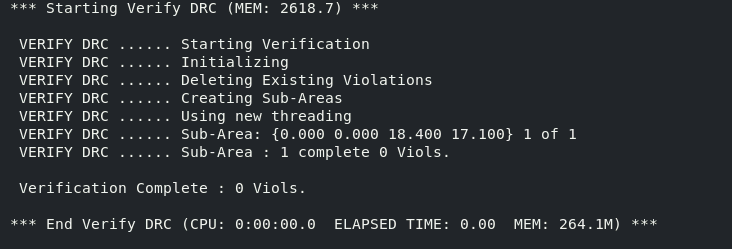
\includegraphics[width=\linewidth]{fig09_alu1_drc}
  \caption{DRC results}\label{fig:alu1drc}
\end{subfigure}\hfill
\begin{subfigure}{0.48\linewidth}\centering
  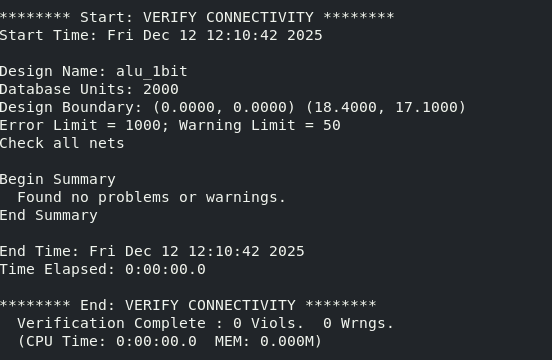
\includegraphics[width=\linewidth]{fig10_alu1_conn}
  \caption{Connectivity check}\label{fig:alu1conn}
\end{subfigure}
\caption{Physical signoff of the 1-bit ALU: (a) design-rule check and
(b) connectivity verification both pass.}
\label{fig:alu1sign}
\end{figure}

\section{Timing and maximum speed}
Post-synthesis static timing analysis reports a critical data-path delay
of \textbf{\SI{3.881}{\nano\second}} through the slice
(\cref{fig:alu1timing}). The path runs from \code{sel\_i[1]} through the
arithmetic multiplexer and full adder to the output. Taking the reciprocal
of the logic delay gives an estimated maximum operating frequency of
\begin{equation}
  f_{\max} \approx \frac{1}{\SI{3.881}{\nano\second}}
           \approx \SI{257}{\mega\hertz},
\end{equation}
with the caveat that this is a relaxed-corner synthesis estimate and that
the reported arrival time includes a large output driver charging the
test load. All paths meet timing with large positive slack against the
(intentionally slow) \SI{1}{\micro\second} analysis clock.

\reportfig{0.85}{fig11_alu1_timing}{Genus timing report for the 1-bit ALU;
the critical path traverses the arithmetic mux and full adder.}
{fig:alu1timing}

\chapter{Part 2a --- 32-bit Hierarchical ALU}
\label{ch:part2a}

The first 32-bit realisation is \emph{structural}: it instantiates
thirty-two copies of the verified 1-bit slice and wires their carries into
a ripple chain. This is the direct expression of the bit-slice methodology
and is the design ultimately chosen for the chip.

\section{Bit-slice chaining}
\Cref{fig:chain} shows the construction. Slice~$i$ takes operand bits
$A_i$, $B_i$ and the carry $C_i$ from the slice below, and produces result
bit $F_i$ and the carry $C_{i+1}$ for the slice above. The external
\bus{Cin} enters slice~0; the final carry $C_{32}$ becomes \bus{Cout}. The
same \sel{} bus fans out to every slice, so all slices perform the same
operation on their respective bit.

\begin{figure}[htbp]
\centering
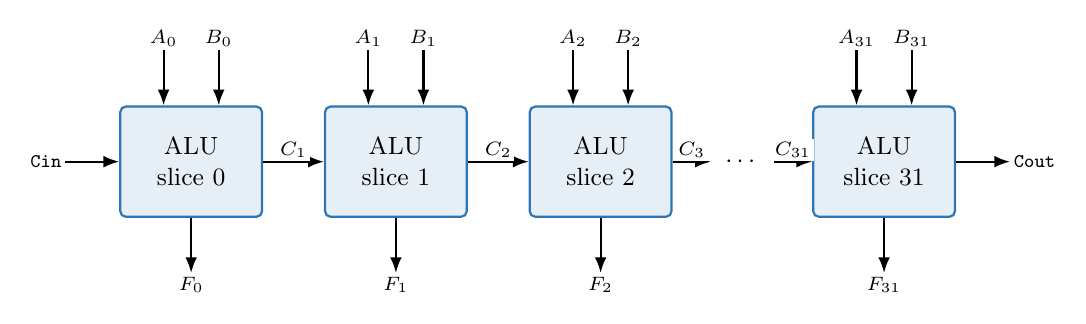
\begin{tikzpicture}[font=\small,node distance=6mm]
  \foreach \i/\x in {0/0, 1/2.6, 2/5.2}{
    \node[arith,minimum width=18mm,minimum height=14mm] (s\i) at (\x,0)
         {ALU\\ slice \i};
  }
  \node at (7.0,0) {$\cdots$};
  \node[arith,minimum width=18mm,minimum height=14mm] (s31) at (8.8,0)
       {ALU\\ slice 31};

  % Carry chain (left to right)
  \draw[sig] (-1.6,0) node[left,buslbl]{Cin} -- (s0.west);
  \draw[sig] (s0.east) -- node[above,buslbl]{$C_1$} (s1.west);
  \draw[sig] (s1.east) -- node[above,buslbl]{$C_2$} (s2.west);
  \draw[sig] (s2.east) -- node[above,buslbl]{$C_3$} (6.6,0);
  \draw[sig] (7.4,0) -- node[above,buslbl]{$C_{31}$} (s31.west);
  \draw[sig] (s31.east) -- (10.4,0) node[right,buslbl]{Cout};

  % Operand inputs (top) and results (bottom)
  \foreach \i in {0,1,2,31}{
    \draw[sig] ($(s\i.north)+(-0.35,0.7)$) node[above,buslbl]{$A_{\i}$}
          -- ($(s\i.north)+(-0.35,0)$);
    \draw[sig] ($(s\i.north)+(0.35,0.7)$) node[above,buslbl]{$B_{\i}$}
          -- ($(s\i.north)+(0.35,0)$);
    \draw[sig] (s\i.south) -- ($(s\i.south)+(0,-0.7)$)
          node[below,buslbl]{$F_{\i}$};
  }
\end{tikzpicture}
\caption{Ripple-carry chaining of thirty-two 1-bit ALU slices. The carry
propagates left-to-right from \bus{Cin} to \bus{Cout}; \sel{} (not shown)
broadcasts to all slices.}
\label{fig:chain}
\end{figure}

\lstinputlisting[style=vlog,firstline=1,lastline=14,
  caption={\texttt{alu\_32bit.v} --- port list, carry vector and the first
  slice instance (slices 1--31 are identical, indices incremented).},
  label={lst:alu32}]{rtl/alu_32bit.v}

The shift operations are handled once at the top level rather than inside
each slice: when \code{S3\,S2}$=10$ or $11$ the 32-bit result is
\code{a\_i>>1} or \code{a\_i<<1} and \bus{Cout} is forced to $0$, exactly
mirroring the per-slice output mux of \cref{fig:alu1top} but applied to the
whole word.

\paragraph{Design decision --- ripple carry.}
Chaining the slice carries produces a \emph{ripple-carry adder}: simple,
compact, and a perfect fit for the bit-slice structure, but with a carry
that must propagate through all 32 stages in the worst case. As the timing
results below confirm, this carry chain is the critical path of the
design --- the classic area-versus-speed trade-off of ripple carry against
carry-lookahead.

\section{Functional simulation}
The 32-bit structural ALU is simulated with wide operands across all
operation classes; \cref{fig:hiersim} shows the result matching the
expected arithmetic, logic and shift outputs.

\reportfig{0.95}{fig12_hier_sim}{32-bit hierarchical ALU simulation, built
from thirty-two 1-bit slices.}{fig:hiersim}

\section{Synthesis}
Genus synthesises the structural design to \textbf{367 cells}
(\cref{fig:hiersynth}). \Cref{tab:hierarea} summarises the area; the
thirty-two \texttt{ADDFX1} full adders ($\SI{164.2}{\micro\meter\squared}$)
are the arithmetic backbone, and clock/DRC buffers again make up a large
share.

\reportfig{0.95}{fig13_hier_synth}{Genus synthesis schematic of the 32-bit
hierarchical ALU (367 leaf cells, 32 slice modules).}{fig:hiersynth}

\begin{table}[htbp]
\centering
\caption{32-bit hierarchical ALU area breakdown (Genus).}
\label{tab:hierarea}
\small
\begin{tabular}{@{}l r r r@{}}
\toprule
Type & Instances & Area (\umsq) & Share \\
\midrule
Inverter & 35  & 24.282  & \SI{2.5}{\percent}\\
Buffer   & 65  & 325.584 & \SI{33.4}{\percent}\\
Logic    & 267 & 625.586 & \SI{64.1}{\percent}\\
\midrule
\textbf{Total} & \textbf{367} & \textbf{975.452} & \SI{100}{\percent}\\
\bottomrule
\end{tabular}
\end{table}

\reportfig{0.55}{fig14_hier_area}{Genus area report, 32-bit hierarchical
ALU.}{fig:hierarea}

\section{Power}
Estimated total power is \textbf{\SI{25.32}{\micro\watt}}
(\cref{fig:hierpower}), again dominated by switching activity.

\reportfig{0.75}{fig15_hier_power}{Genus power report, 32-bit hierarchical
ALU.}{fig:hierpower}

\section{Place and route}
\Cref{fig:hierpnr} shows the placed-and-routed core in Innovus.

\reportfig{0.6}{fig16_hier_pnr}{Innovus place-and-route of the 32-bit
hierarchical ALU.}{fig:hierpnr}

\section{Physical verification}
\begin{figure}[htbp]
\centering
\begin{subfigure}{0.48\linewidth}\centering
  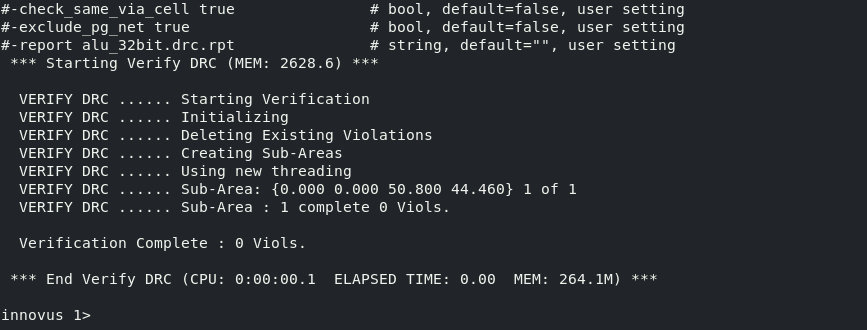
\includegraphics[width=\linewidth]{fig17_hier_drc}
  \caption{DRC results}\label{fig:hierdrc}
\end{subfigure}\hfill
\begin{subfigure}{0.48\linewidth}\centering
  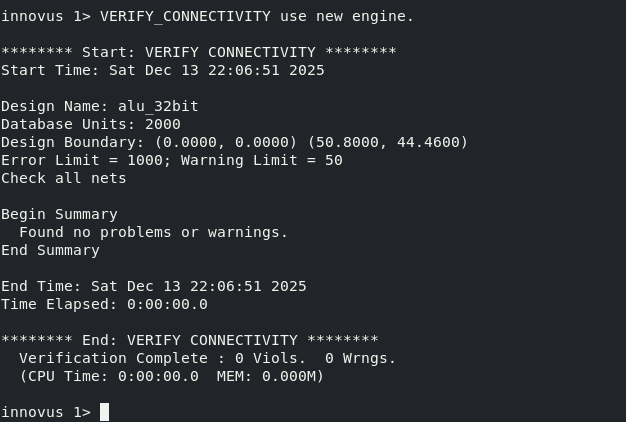
\includegraphics[width=\linewidth]{fig18_hier_conn}
  \caption{Connectivity check}\label{fig:hierconn}
\end{subfigure}
\caption{Physical signoff of the 32-bit hierarchical ALU: DRC and
connectivity both clean.}
\label{fig:hiersign}
\end{figure}

\section{Timing and maximum speed}
Static timing analysis reports a worst-case critical path of
\textbf{\SI{9.724}{\nano\second}}. As anticipated, the path runs through
the \textbf{ripple-carry chain}: from an early select/operand bit, through
the arithmetic mux of slice~0, and then \code{CI}$\rightarrow$\code{CO}
across all thirty-two \texttt{ADDFX1} adders to \code{f\_o[31]}. Each adder
stage contributes roughly \SI{186}{\pico\second} of carry delay, so the
32-stage chain dominates. The estimated maximum frequency is
\begin{equation}
  f_{\max} \approx \frac{1}{\SI{9.724}{\nano\second}}
           \approx \SI{102.8}{\mega\hertz}.
\end{equation}
This ripple-carry delay is the price of the simple, highly regular
bit-slice structure, and it is the number carried into the comparison of
\cref{ch:compare}.

\chapter{Part 2b --- 32-bit Behavioural ALU}
\label{ch:part2b}

The second 32-bit realisation describes the same functionality in a single
\emph{behavioural} module. Instead of instantiating slices, it models the
operations directly on 32-bit vectors and lets the synthesiser infer the
datapath. This chapter mirrors the flow of \cref{ch:part2a} so the two can
be compared cleanly in \cref{ch:compare}.

\section{Behavioural description}
A single \code{always @*} block with a \code{casez} on \sel{} maps each
opcode to a vector expression (\cref{lst:behav}). A 33-bit temporary
captures the carry-out of the arithmetic operations, and explicit defaults
avoid inferred latches.

\lstinputlisting[style=vlog,firstline=1,lastline=45,
  caption={\texttt{alu\_32bit\_behavioral.v} --- ports and the arithmetic
  branches of the \texttt{casez} (logic/shift branches follow the same
  pattern).},label={lst:behav}]{rtl/alu_32bit_behavioral.v}

\paragraph{Design decision --- behavioural vs.\ structural.}
The behavioural style is far shorter and easier to write and read: the
subtract branch is literally \code{a + \~{}b + cin}, and the increment,
decrement and shift branches are one line each. The cost is control over
the resulting hardware. Because each arithmetic branch is an independent
\code{+} expression, the synthesiser infers \emph{several} adders rather
than reusing one, which --- as the area report shows --- makes this design
substantially larger than the hierarchical one. The structural design
trades brevity for a smaller, more predictable datapath.

\section{Functional simulation}
The behavioural ALU is simulated over the same operation set; the waveform
in \cref{fig:behavsim} confirms functional equivalence with the structural
design.

\reportfig{0.95}{fig19_behav_sim}{32-bit behavioural ALU simulation
waveform.}{fig:behavsim}

\section{Synthesis}
Genus synthesises the behavioural design to \textbf{635 cells}
(\cref{fig:behavsynth,tab:behavarea}) --- notably it infers \textbf{64}
\texttt{ADDFX1} plus \texttt{ADDHX1} adders, twice the arithmetic hardware
of the structural version, because the separate \code{+} expressions are
not shared.

\reportfig{0.95}{fig20_behav_synth}{Genus synthesis schematic of the 32-bit
behavioural ALU.}{fig:behavsynth}

\begin{table}[htbp]
\centering
\caption{32-bit behavioural ALU area breakdown (Genus).}
\label{tab:behavarea}
\small
\begin{tabular}{@{}l r r r@{}}
\toprule
Type & Instances & Area (\umsq) & Share \\
\midrule
Inverter & 58  & 40.014   & \SI{2.7}{\percent}\\
Buffer   & 67  & 329.004  & \SI{22.1}{\percent}\\
Logic    & 510 & 1117.998 & \SI{75.2}{\percent}\\
\midrule
\textbf{Total} & \textbf{635} & \textbf{1487.016} & \SI{100}{\percent}\\
\bottomrule
\end{tabular}
\end{table}

\reportfig{0.5}{fig21_behav_area}{Genus area report, 32-bit behavioural
ALU.}{fig:behavarea}

\section{Power}
Estimated total power is \textbf{\SI{22.29}{\micro\watt}}
(\cref{fig:behavpower}) --- slightly lower than the structural design
despite the larger area, because the redundant adders are not all
switching simultaneously for a given operation.

\reportfig{0.75}{fig22_behav_power}{Genus power report, 32-bit behavioural
ALU.}{fig:behavpower}

\section{Place and route}
\reportfig{0.6}{fig23_behav_pnr}{Innovus place-and-route of the 32-bit
behavioural ALU.}{fig:behavpnr}

\section{Physical verification}
\begin{figure}[htbp]
\centering
\begin{subfigure}{0.48\linewidth}\centering
  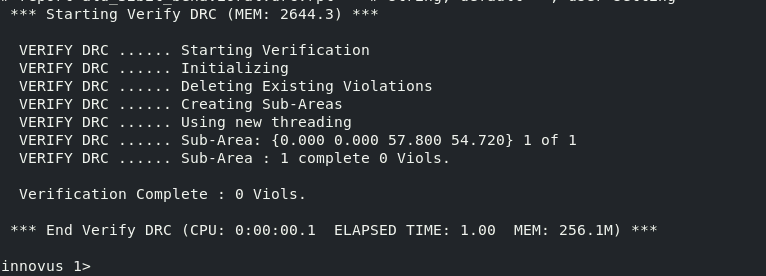
\includegraphics[width=\linewidth]{fig24_behav_drc}
  \caption{DRC results}\label{fig:behavdrc}
\end{subfigure}\hfill
\begin{subfigure}{0.48\linewidth}\centering
  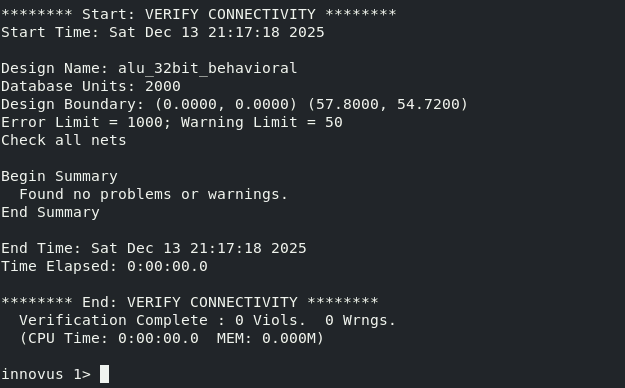
\includegraphics[width=\linewidth]{fig25_behav_conn}
  \caption{Connectivity check}\label{fig:behavconn}
\end{subfigure}
\caption{Physical signoff of the 32-bit behavioural ALU.}
\label{fig:behavsign}
\end{figure}

\section{Timing and maximum speed}
The behavioural design's critical path is \textbf{\SI{9.832}{\nano\second}},
essentially identical to the structural design and again dominated by a
32-stage carry ripple (the inferred adder/incrementer chain
\code{addinc\_add\_29\_48\_*}). The estimated maximum frequency is
\begin{equation}
  f_{\max} \approx \frac{1}{\SI{9.832}{\nano\second}}
           \approx \SI{101.7}{\mega\hertz}.
\end{equation}
So the two 32-bit designs are matched on speed but --- as
\cref{ch:compare} shows --- not on area.

\chapter{Comparison and Core Selection}
\label{ch:compare}

The assignment requires the two 32-bit cores to be compared and the
smaller one carried forward to chip integration. This chapter consolidates
the synthesis results and justifies the choice.

\section{Consolidated results}
\Cref{tab:compare} gathers the area, power and timing figures for all
three designs. The 1-bit slice is included for reference; the decision is
between the two 32-bit cores.

\begin{table}[htbp]
\centering
\caption{Synthesis comparison (Genus, \texttt{gsclib045},
\texttt{PVT\_0P9V\_125C}).}
\label{tab:compare}
\small
\begin{tabularx}{\linewidth}{@{}X r r r@{}}
\toprule
Metric & 1-bit slice & \makecell[r]{32-bit\\hierarchical (2a)} &
\makecell[r]{32-bit\\behavioural (2b)}\\
\midrule
Standard cells        & 12     & 367     & 635\\
Total area (\umsq)     & 39.67  & 975.45  & 1487.02\\
\quad buffers (\umsq)   & 16.42  & 325.58  & 329.00\\
\quad logic (\umsq)     & 22.57  & 625.59  & 1118.00\\
Total power (\si{\micro\watt}) & 0.998 & 25.32 & 22.29\\
Critical path (\si{\nano\second}) & 3.881 & 9.724 & 9.832\\
Est.\ $f_{\max}$ (\si{\mega\hertz}) & $\approx$257 & $\approx$103 & $\approx$102\\
\bottomrule
\end{tabularx}
\end{table}

\begin{figure}[htbp]
\centering
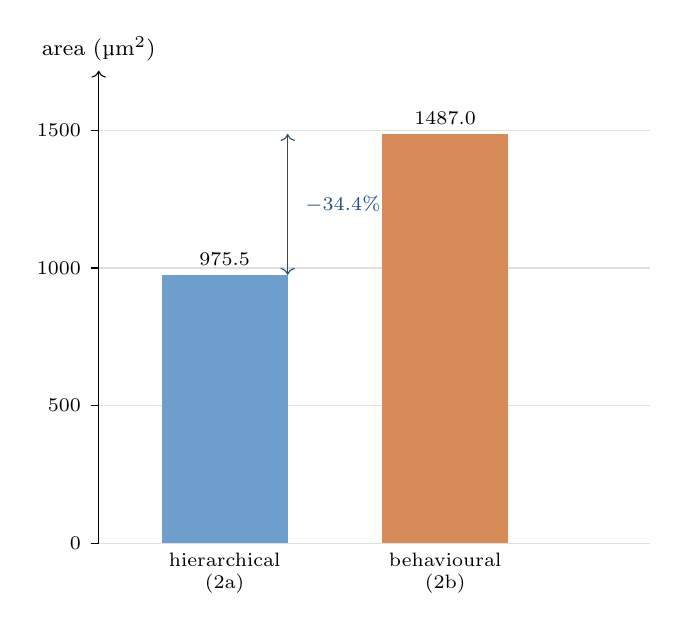
\begin{tikzpicture}[font=\small]
  \def\scale{0.0035}
  % axis
  \draw[->] (0,0) -- (0,6) node[above,font=\footnotesize]{area (\umsq)};
  \foreach \y in {0,500,1000,1500}{
    \draw (0,{\y*\scale}) -- (-0.1,{\y*\scale}) node[left,font=\scriptsize]{\y};
    \draw[gray!25] (0,{\y*\scale}) -- (7,{\y*\scale});
  }
  % bars
  \fill[arithblk!70] (0.8,0) rectangle (2.4,{975.452*\scale});
  \node[above,font=\scriptsize] at (1.6,{975.452*\scale}) {975.5};
  \node[below,align=center,font=\scriptsize] at (1.6,0)
       {hierarchical\\(2a)};
  \fill[padblk!70] (3.6,0) rectangle (5.2,{1487.016*\scale});
  \node[above,font=\scriptsize] at (4.4,{1487.016*\scale}) {1487.0};
  \node[below,align=center,font=\scriptsize] at (4.4,0)
       {behavioural\\(2b)};
  % delta annotation
  \draw[<->,accent] (2.4,{975.452*\scale}) -- (2.4,{1487.016*\scale});
  \node[right,accent,font=\scriptsize,align=left] at (2.5,{1231*\scale})
       {$-34.4\%$};
\end{tikzpicture}
\caption{Core-area comparison. The hierarchical design is
\SI{34.4}{\percent} smaller than the behavioural design
(\SI{975.5}{\micro\meter\squared} vs \SI{1487.0}{\micro\meter\squared}).}
\label{fig:areacompare}
\end{figure}

\section{Discussion}
\begin{description}[leftmargin=1.6em,style=nextline]
  \item[Area] The hierarchical core is \SI{34.4}{\percent} smaller
        (\cref{fig:areacompare}). The behavioural code writes each
        arithmetic operation as an independent \code{+}, so the
        synthesiser infers about twice the adder hardware
        (64 vs 32 full adders) and cannot share it; operand-mux reuse in
        the structural design keeps its datapath lean.
  \item[Speed] The two are effectively tied
        (\SI{9.72}{\nano\second} vs \SI{9.83}{\nano\second}); both are
        limited by a 32-stage ripple carry, so neither style wins on the
        critical path.
  \item[Power] The behavioural design draws marginally less total power
        (\SI{22.29}{} vs \SI{25.32}{\micro\watt}) despite its larger area,
        because its redundant adders are not all active for any single
        operation --- a small effect that does not offset the area gap.
\end{description}

\section{Selected core}
\begin{center}
\fbox{\parbox{0.92\linewidth}{\centering
The \textbf{32-bit hierarchical (structural) core} is selected for chip
integration: it is \SI{34.4}{\percent} smaller than the behavioural core
and marginally faster, at equivalent functionality.}}
\end{center}
\noindent
Its GDSII (\code{alu\_32bit.gds}) is streamed out of Innovus and imported
into Virtuoso for pad-frame assembly in \cref{ch:pad}.

\chapter{Pad Frame and Chip Integration}
\label{ch:pad}

The final flow step turns the routed core into a complete chip. The
selected hierarchical core (\cref{ch:compare}) is streamed out as GDSII and
imported into Cadence Virtuoso, where it is placed inside a provided
\textbf{pad frame} --- the ring of I/O pads that connects the internal
signals to the outside world (bond wires / package). This chapter
documents the pad plan, the pad-to-signal wiring, and the assembled
layout.

\section{Pad plan}
The chip uses a \textbf{104-signal} pad ring with \textbf{26 pads on each
of the four edges}. Grouping the buses by edge keeps the core-to-pad
routing short and untangled: the 32-bit \bus{A} and \bus{B} operands enter
from the top and left, the 32-bit \bus{F} result leaves from the right and
bottom, and the control signals sit together on the bottom edge.
\Cref{fig:padring} shows the arrangement and \cref{tab:pinmap} gives the
exact per-edge assignment taken from the Innovus pin-assignment file
(\code{pinAssignment.io}).

\begin{figure}[htbp]
\centering
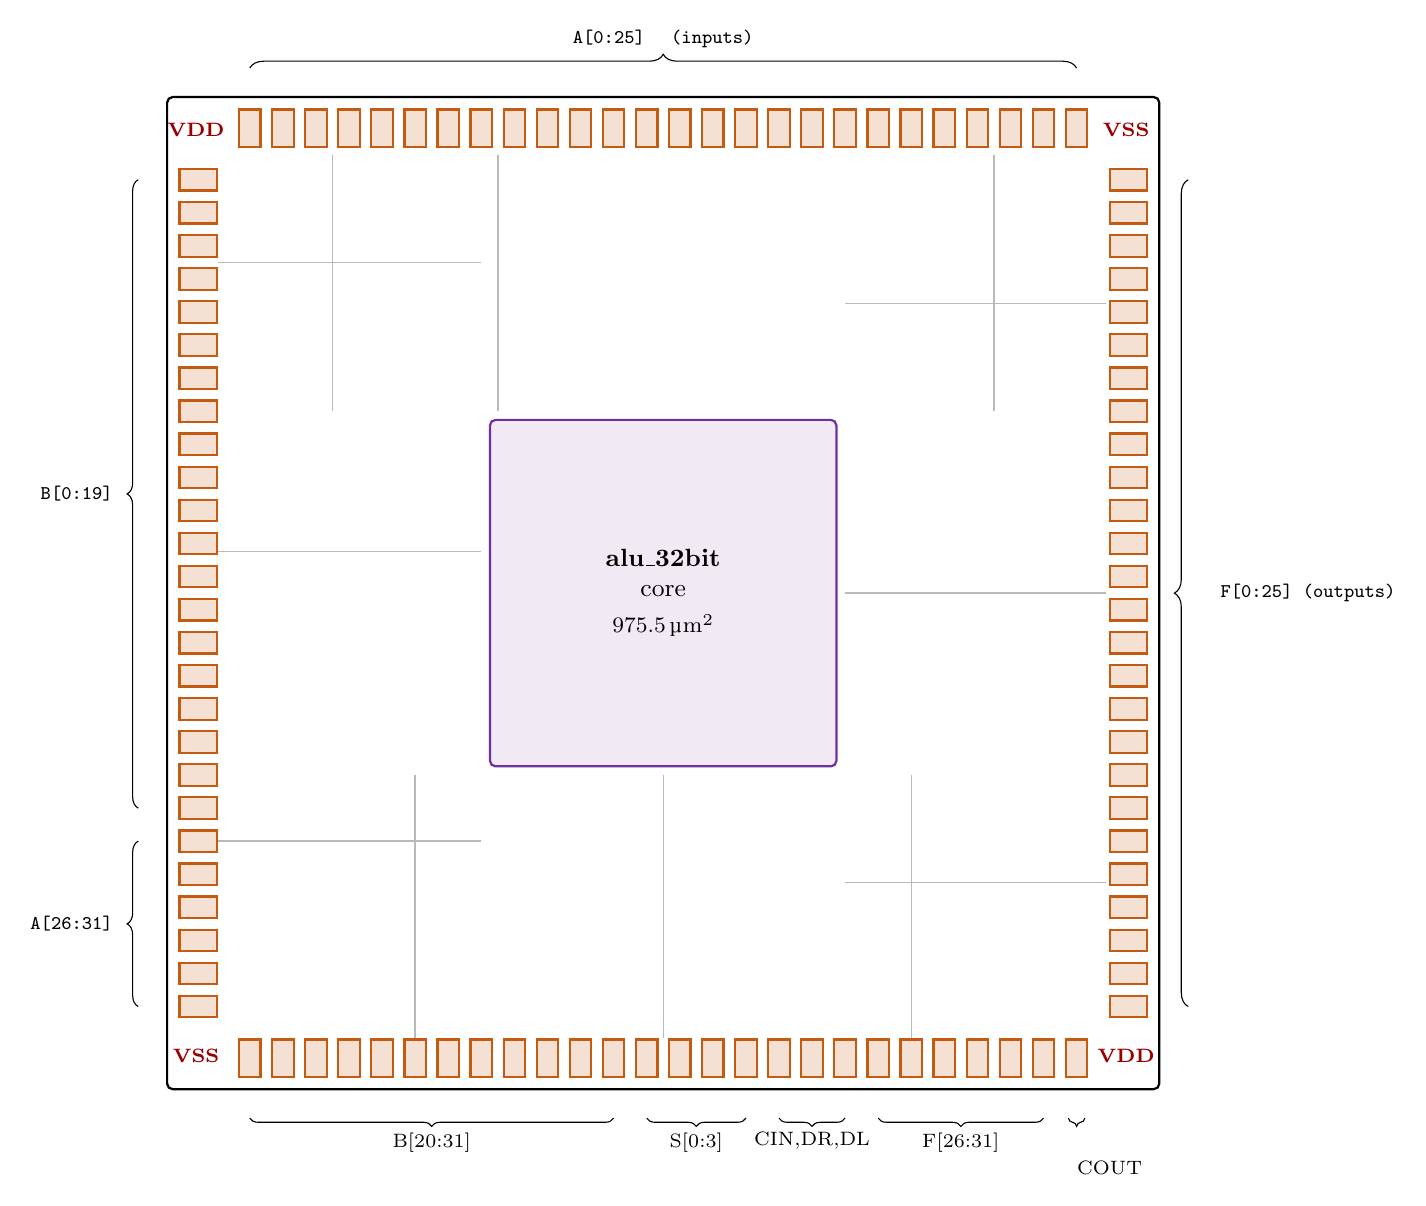
\begin{tikzpicture}[font=\small,scale=1.05]
  % Die outline
  \draw[thick,rounded corners=2pt] (0,0) rectangle (12,12);
  % Core
  \node[core,minimum width=44mm,minimum height=44mm] (core) at (6,6)
      {\bfseries alu\_32bit\\ core\\[2pt]
       {\footnotesize\SI{975.5}{\micro\meter\squared}}};

  % Pad ticks on the four edges (26 per edge)
  \foreach \i in {0,...,25}{
    \pgfmathsetmacro{\p}{1+\i*10/25}
    \fill[pad] ({\p-0.13},11.4) rectangle ({\p+0.13},11.85); % top
    \fill[pad] ({\p-0.13},0.15) rectangle ({\p+0.13},0.6);   % bottom
    \fill[pad] (0.15,{\p-0.13}) rectangle (0.6,{\p+0.13});   % left
    \fill[pad] (11.4,{\p-0.13}) rectangle (11.85,{\p+0.13}); % right
  }
  % Corner power pads
  \foreach \x/\y/\l in {0.35/11.6/VDD, 11.6/11.6/VSS,
                        0.35/0.4/VSS, 11.6/0.4/VDD}
    \node[font=\scriptsize\bfseries,text=red!60!black] at (\x,\y) {\l};

  % Example core-to-pad routing (illustrative)
  \foreach \a/\b in {2/11.4, 4/11.4, 10/11.4}
    \draw[gray!55,line width=0.5pt] (\a,8.2) -- (\a,11.3);
  \foreach \a/\b in {3/8.2, 6/8.2, 9/8.2}
    \draw[gray!55,line width=0.5pt] (\a,3.8) -- (\a,0.62);
  \foreach \a in {2.5,6,9.5}
    \draw[gray!55,line width=0.5pt] (8.2,\a) -- (11.35,\a);
  \foreach \a in {3,6.5,10}
    \draw[gray!55,line width=0.5pt] (3.8,\a) -- (0.62,\a);

  % ---- Group braces + labels ----
  % TOP : A[0:25]
  \draw[decorate,decoration={brace,amplitude=5pt}] (1,12.35) -- (11,12.35);
  \node[above=6pt,buslbl] at (6,12.35) {\bfseries A[0:25] \; (inputs)};
  % RIGHT : F[0:25]
  \draw[decorate,decoration={brace,amplitude=5pt,mirror}]
        (12.35,11) -- (12.35,1);
  \node[right=6pt,buslbl] at (12.5,6) {\bfseries F[0:25] (outputs)};
  % LEFT : lower A[26:31], upper B[0:19]
  \draw[decorate,decoration={brace,amplitude=4pt}] (-0.35,1) -- (-0.35,3);
  \node[left=5pt,buslbl,align=right] at (-0.45,2) {A[26:31]};
  \draw[decorate,decoration={brace,amplitude=4pt}] (-0.35,3.4) -- (-0.35,11);
  \node[left=5pt,buslbl,align=right] at (-0.45,7.2) {B[0:19]};
  % BOTTOM groups
  \draw[decorate,decoration={brace,amplitude=3pt,mirror}] (1,-0.35) -- (5.4,-0.35);
  \node[below=4pt,buslbl,font=\scriptsize] at (3.2,-0.35) {B[20:31]};
  \draw[decorate,decoration={brace,amplitude=3pt,mirror}] (5.8,-0.35) -- (7.0,-0.35);
  \node[below=4pt,buslbl,font=\scriptsize] at (6.4,-0.35) {S[0:3]};
  \draw[decorate,decoration={brace,amplitude=3pt,mirror}] (7.4,-0.35) -- (8.2,-0.35);
  \node[below=4pt,buslbl,font=\scriptsize] at (7.8,-0.35) {CIN,DR,DL};
  \draw[decorate,decoration={brace,amplitude=3pt,mirror}] (8.6,-0.35) -- (10.6,-0.35);
  \node[below=4pt,buslbl,font=\scriptsize] at (9.6,-0.35) {F[26:31]};
  \draw[decorate,decoration={brace,amplitude=3pt,mirror}] (10.9,-0.35) -- (11.1,-0.35);
  \node[below=4pt,buslbl,font=\scriptsize] at (11.4,-0.7) {COUT};
\end{tikzpicture}
\caption{Pad-frame plan for the 32-bit ALU chip: 104 signal pads, 26 per
edge. Operands \bus{A}/\bus{B} enter from the top and left, result \bus{F}
leaves from the right and bottom, and controls (\bus{S}, \bus{Cin},
\bus{DR}, \bus{DL}, \bus{Cout}) occupy the bottom edge. Grey lines
illustrate representative core-to-pad routing; corner pads carry
\bus{VDD}/\bus{VSS}.}
\label{fig:padring}
\end{figure}

\begin{table}[htbp]
\centering
\caption{Per-edge pad assignment (from \code{pinAssignment.io}, Metal-4
pins). 104 signal pads in total.}
\label{tab:pinmap}
\small
\begin{tabularx}{\linewidth}{@{}l l c X@{}}
\toprule
Edge & Signals & Pads & Notes\\
\midrule
Top    & \bus{A[0:25]}                       & 26 & operand \bus{A}, low half \\
Left   & \bus{A[26:31]}, \bus{B[0:19]}       & 26 & rest of \bus{A}, start of \bus{B} \\
Bottom & \bus{B[20:31]}, \bus{S[0:3]}, \bus{CIN}, \bus{DR}, \bus{DL}, \bus{F[26:31]}, \bus{COUT}
                                             & 26 & controls + high result bits \\
Right  & \bus{F[0:25]}                       & 26 & result \bus{F}, low half \\
\midrule
\multicolumn{2}{@{}l}{\textbf{Total signal pads}} & \textbf{104} &
  \bus{VDD}/\bus{VSS} supplied by the pad frame \\
\bottomrule
\end{tabularx}
\end{table}

\paragraph{Design note --- the shift serial pads.}
The pad plan reserves two pads, \bus{DR} and \bus{DL}, for the shift
serial inputs \bus{Din,R}/\bus{Din,L} of the specification. In the RTL as
implemented the shift result is derived internally from \bus{A}
(\code{a>>1}/\code{a<<1}), so these two pads are provided for
specification completeness but are not driven into the core. Wiring them
to the shift-in position of the datapath is a natural extension.

\section{Assembled chip layout}
The routed core GDSII is placed inside the pad frame in Virtuoso and the
pads are wired to the corresponding core pins. \Cref{fig:chippad} shows the
assembled full-chip layout; \cref{fig:chippin} is the corresponding pin
(bond) diagram.

\begin{figure}[htbp]
\centering
\begin{subfigure}{0.52\linewidth}\centering
  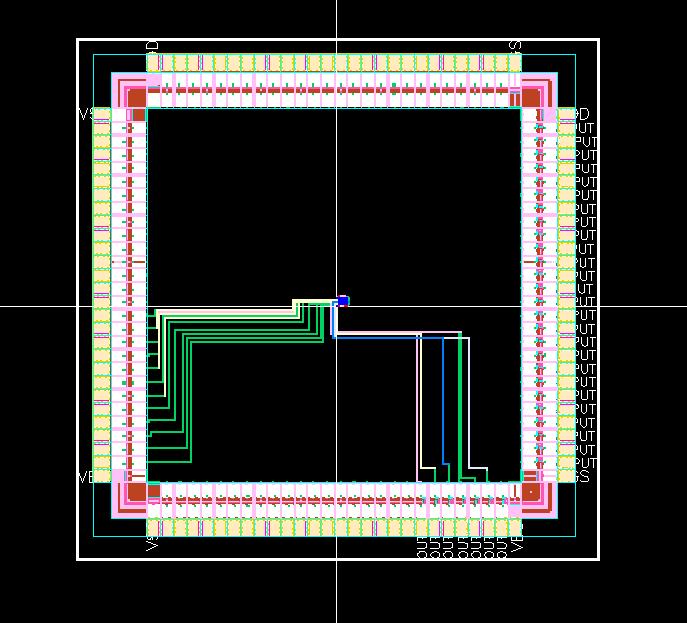
\includegraphics[width=\linewidth]{fig26_chip_padframe}
  \caption{Full-chip layout: core inside the pad frame.}
  \label{fig:chippad}
\end{subfigure}\hfill
\begin{subfigure}{0.44\linewidth}\centering
  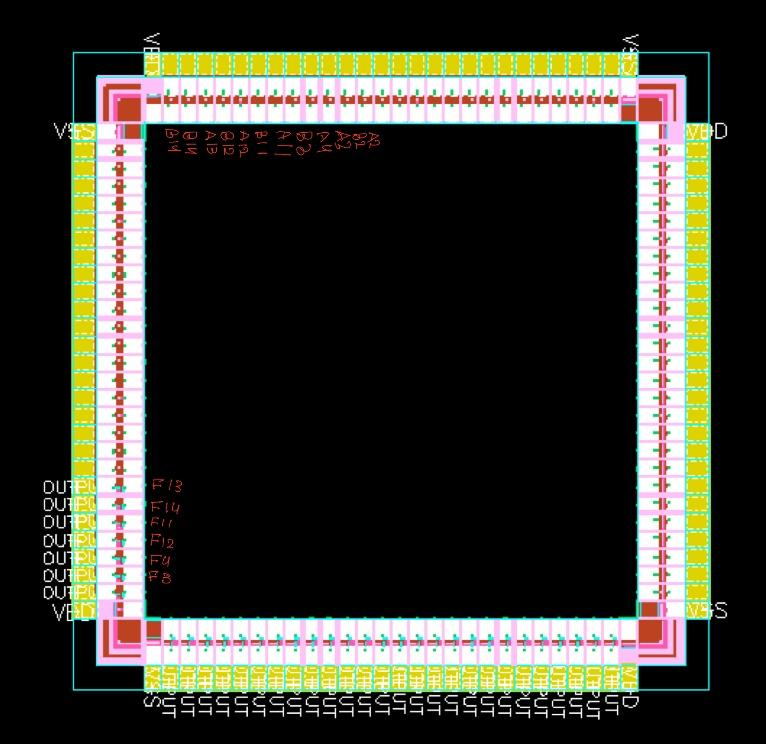
\includegraphics[width=\linewidth]{fig27_chip_pindiagram}
  \caption{Chip pin/bond diagram.}
  \label{fig:chippin}
\end{subfigure}
\caption{Virtuoso assembly of the hierarchical 32-bit ALU into the pad
frame. The green/pink traces in (a) are the completed core-to-pad
connections.}
\label{fig:chip}
\end{figure}

\paragraph{Status of the wiring.}
As seen in \cref{fig:chippad}, the core is correctly placed in the frame
and a subset of the I/O nets (visible in the lower-left) are wired to their
pads, but \emph{not all} 104 connections were completed within the project
time budget. The pad plan, pin assignment and routing methodology are
fully defined (\cref{fig:padring}, \cref{tab:pinmap}); completing the
remaining pad connections and re-running DRC/LVS on the full chip is the
final step to a tape-out-ready layout.

\chapter{Conclusion}
\label{ch:conc}

\section{Summary}
A 32-bit Arithmetic-Logic Unit was designed and carried through the
complete Cadence RTL-to-GDS flow on the GPDK045 \SI{45}{\nano\meter} CMOS
process. Following a bit-slice methodology, a 1-bit ALU slice was designed,
exhaustively verified, synthesised and physically implemented; thirty-two
slices were then chained into a 32-bit ALU. A behavioural 32-bit design was
implemented in parallel for comparison. \Cref{tab:final} recaps the
headline results.

\begin{table}[htbp]
\centering
\caption{Final results at a glance.}
\label{tab:final}
\small
\begin{tabularx}{\linewidth}{@{}X r r r@{}}
\toprule
& 1-bit slice & \makecell[r]{32-bit\\hierarchical} &
  \makecell[r]{32-bit\\behavioural}\\
\midrule
Cells                       & 12    & 367    & 635\\
Area (\umsq)                 & 39.67 & 975.45 & 1487.02\\
Power (\si{\micro\watt})     & 0.998 & 25.32  & 22.29\\
Critical path (\si{\nano\second}) & 3.881 & 9.724 & 9.832\\
$f_{\max}$ (\si{\mega\hertz}) & $\approx$257 & $\approx$103 & $\approx$102\\
DRC / connectivity          & clean & clean  & clean\\
\bottomrule
\end{tabularx}
\end{table}

The hierarchical core was \SI{34.4}{\percent} smaller than the behavioural
core at equivalent function and speed, so it was selected, streamed out as
GDSII, and placed into a 104-pad, four-edge pad frame in Virtuoso to form
the chip.

\section{Key design decisions}
\begin{itemize}
  \item \textbf{Bit-slice architecture} --- one verified 1-bit cell tiled
        32 times, giving modularity, reuse and low verification effort.
  \item \textbf{Single shared adder per slice} --- add, subtract,
        increment and decrement are realised by multiplexing the adder's
        second operand ($0$, $B$, $\overline{B}$, $1$) with two's
        complement for subtraction.
  \item \textbf{Two-level select} --- \code{S3\,S2} chooses the operation
        class at the output mux, \code{S1\,S0} chooses the specific
        function, keeping every slice identical.
  \item \textbf{Structural over behavioural} --- chosen for
        \SI{34.4}{\percent} smaller area thanks to adder sharing.
  \item \textbf{Worst-case corner} --- signoff on
        \texttt{slow\_vdd1v0} / \texttt{PVT\_0P9V\_125C} so timing is
        conservative.
  \item \textbf{Edge-grouped pad plan} --- operands, result and controls
        grouped per edge to minimise core-to-pad routing.
\end{itemize}

\section{Limitations and future work}
\begin{description}[leftmargin=1.6em,style=nextline]
  \item[Ripple-carry critical path] Both 32-bit designs are limited to
        $\approx$\SI{100}{\mega\hertz} by the 32-stage carry ripple.
        Replacing it with a carry-lookahead or carry-select adder would
        cut the critical path at a modest area cost.
  \item[Incomplete pad wiring] The core is placed in the pad frame and a
        subset of I/O nets are wired, but the full 104-pad connection was
        not finished. Completing it and running full-chip DRC/LVS is the
        remaining step to a tape-out-ready layout.
  \item[Unconnected shift pads] \bus{DR}/\bus{DL} are reserved but not
        driven into the datapath; wiring them realises true serial shift.
  \item[Combinational only] The ALU has no registers; embedding it in a
        pipelined datapath would require input/output registers and clock
        distribution (a clock tree, absent here as the design is
        combinational).
\end{description}

\section{Closing}
The project demonstrates the full professional VLSI design experience:
from a specification and Verilog RTL, through simulation, synthesis,
place-and-route, physical verification and GDSII export, to full-chip
integration in a pad frame --- with quantified area, power and timing
trade-offs driving the design decisions at each step.


\appendix
\chapter{RTL Source Listings}
\label{app:rtl}

This appendix contains the complete Verilog source for the designs
documented in the report. The files are copied verbatim into
\code{rtl-to-gds-alu-doc/rtl/} so the document is self-contained; they are
identical to the sources under \code{Part1\_1BitALU/}, \code{Part2a\_32BitALU/}
and \code{Part2b\_32BitALU/} in the repository.

\section{1-bit slice sub-modules}
\lstinputlisting[style=vlog,caption={\texttt{full\_adder.v}}]{rtl/full_adder.v}
\lstinputlisting[style=vlog,caption={\texttt{mux4x1.v}}]{rtl/mux4x1.v}
\lstinputlisting[style=vlog,caption={\texttt{arithmetic\_circuit.v}}]{rtl/arithmetic_circuit.v}
\lstinputlisting[style=vlog,caption={\texttt{logic\_circuit.v}}]{rtl/logic_circuit.v}
\lstinputlisting[style=vlog,caption={\texttt{alu\_1bit.v}}]{rtl/alu_1bit.v}

\section{32-bit hierarchical (structural) ALU}
\lstinputlisting[style=vlog,caption={\texttt{alu\_32bit.v} --- full
listing, all 32 slice instances.}]{rtl/alu_32bit.v}

\section{32-bit behavioural ALU}
\lstinputlisting[style=vlog,caption={\texttt{alu\_32bit\_behavioral.v} ---
full listing.}]{rtl/alu_32bit_behavioral.v}

\chapter{Testbenches}
\label{app:tb}
\lstinputlisting[style=vlog,caption={\texttt{tb\_1bit\_alu.v}}]{rtl/tb_1bit_alu.v}
\lstinputlisting[style=vlog,caption={\texttt{tb\_32bit\_alu.v}}]{rtl/tb_32bit_alu.v}
\lstinputlisting[style=vlog,caption={\texttt{tb\_32bit\_alu\_behavioral.v}}]{rtl/tb_32bit_alu_behavioral.v}


\end{document}
